\documentclass[aps,pra,twocolumn,floatfix,superscriptaddress]{revtex4-1}%,twocolumn,draft
\usepackage{amsmath}
\usepackage{amssymb}
\usepackage{xcolor}
\usepackage{graphicx}
\usepackage{dcolumn}
\usepackage{braket}

\def\boldrm#1{{\bf #1}}
\def\boldit#1{\mbox{\boldmath$#1$}}
\def\calbf#1{\mbox{\boldmath${\cal #1}$}}
\def\q{\quad}
\def\k{\mbox{\boldmath$\kappa$}}
\newcommand{\eq}[1]{Eq.~\eqref{#1}}

\begin{document}

\title{Dynamical signatures of bound states in waveguide QED}

\author{E. S\'anchez-Burillo}
\affiliation{Instituto de Ciencia de Materiales de Aragon and Departamento de Fisica de la Materia Condensada, CSIC-Universidad de Zaragoza, E-50012 Zaragoza, Spain}
\author{D. Zueco}
\affiliation{Instituto de Ciencia de Materiales de Aragon and Departamento de Fisica de la Materia Condensada, CSIC-Universidad de Zaragoza, E-50012 Zaragoza, Spain}
\affiliation{Fundacion ARAID, Paseo Maria Agustin 36, E-50004 Zaragoza, Spain}
\author{L. Mart\'in-Moreno}
\affiliation{Instituto de Ciencia de Materiales de Aragon and Departamento de Fisica de la Materia Condensada, CSIC-Universidad de Zaragoza, E-50012 Zaragoza, Spain}
\author{J. J. Garc\'ia-Ripoll}
\affiliation{Instituto de Fisica Fundamental, IFF-CSIC, Calle Serrano 113b, Madrid E-28006}
\begin{abstract}
We study the spontaneous decay of an impurity coupled to a linear array of bosonic cavities forming a single-band waveguide. The frequency of the emitted photon is different from the single-photon scattering resonance frequency, which perfectly matches the bare frequency of the impurity. This breaks down the correspondence between spontaneous emission and scattering. We study how the position of the impurity energy with respect to the photonic band influences the profile of the emitted photon in position space. In addition, the impurity presents a rich dynamics: it shows an exponential decay up to intermediate times, followed by a power-law tail in the long-time regime, and finally reaches an oscillatory stationary regime.
\end{abstract}

\maketitle

\section{Introduction}

Interaction between few-level systems or quantum impurities and photonic media with nonlinear dispersion relations and band gaps gives rise to a plethora of interesting phenomena \cite{Lambropoulos2000}. Examples are the modification of the level structure of the impurity \cite{John1990,John1991,Ripoll2015}, non-trivial dynamics \cite{Khalfin1958,Fonda1978,Hack1982,John1994,Gaveau1995,Garmon2013,Redchenko2014,Lombardo2014}, and charge transfer enhancement \cite{Tanaka2006}. %
A characteristic phenomenon is the appearance of bound states\ \cite{John1984,John1987} where a photonic excitation is confined to the vicinity of the impurity. This idea has been studied in various theoretical works, finding phenomena such as decoherence suppression \cite{Tong2010a}, preservation of quantum correlations \cite{Tong2010b,Yang2013,Lu2013} or existence of multi-photon bound states\ \cite{Cirac2015,Calajo2016}. {\color{blue}Quite recently, all these calculations have had a renewal relevance due to the development of different experimental layouts where the dynamics of the bound states with an impurity at the single-photon limit is accessible. Examples are photonic crystals \cite{Arcari2014,Sollner2015,Lodahl2015}, cold atoms \cite{goban2015,thompson2013}, and circuit QED systems \cite{Astafiev2010,Hoi2011,Hoi2013,VanLoo2013,Hoi2013b,Liu2017}.

We choose a prototypical model in waveguide-QED where an impurity is coupled to a bosonic medium. The latter is a bosonic tight-binding model with a cosine-shaped band. Due to the finite width of the band, two bound states appear around the impurity. 

In this work, we study the consequences of the appearance of the bound states in a spontaneous decay situation. This problem has already been treated in the literature when the energy of the impurity is in the middle of the band \cite{Lombardo2014} or when it is close to its inferior limit, so the superior limit of the band can be neglected \cite{Garmon2013}. We solve it for general values of the parameters, which are the energy of the impurity with respect to the the band and the coupling between the impurity and the photonic medium compared to the bandwidth. This allows to find an energy shift of the emitted photon with respect to the energy of the impurity, provided the latter is not in the middle of the band. This phenomenon breaks the usual correspondence between scattering and emission spectra, since the former presents a resonance as the energy of the incident photon matches with the energy of the impurity \cite{Nori2008a, Fan2005a, Fan2005b}. Secondly, we study the profile of the emitted field in position space, finding differences with respect to a photonic medium with a linear dispersion relation. Lastly, we characterize the dynamics of the impurity: it decays exponentially with a decay rate different from that given by the Fermi's golden rule, it presents an algebraic decay due to the presence of singularities in the density of photonic states, and it eventually follows a stationary oscillating regime.}

%The purpose of this paper is to study the decay of a quantum impurity embedded in a photonic reservoir with a band gap. More precisely, we consider a waveguide-QED scenario, where the medium is a one-dimensional array of coupled bosonic cavities with tight-binding interaction. This model gives a cosine-shaped dispersion relation for propagating photons and bound states around the impurity. We find that the excited impurity emits a photon with an energy shift with respect to the energy of the impurity, which depends on the coupling constant and the position of the energy of the impurity with respect to the band. We show the impurity presents a complex time evolution, comprising exponential, power law and oscillatory regimes. Lastly, we have studied the profile of the field in the position space

The manuscript is organized as follows. First, we introduce the Hamiltonian and its spectrum in the single-excitation subspace.  In section \ref{sec:scatt} we briefly review the single-photon scattering. In section \ref{sec:spontaneous_decay}, we discuss the main results of the paper. First, we present the already mentioned frequency shift of the emitted photon as a function of the coupling constant and the energy of the impurity. Then, we study the field distribution of the emitted photon in position space. We next characterize the spontaneous emission of the impurity.
We end up with the conclusions. Some technical details are described in the appendices.


%%%%%%%%%%%%%%%%%%
%%%%%%%%%%%%%%%%%%
%%%%% Model
%%%%%%%%%%%%%%%%%%
%%%%%%%%%%%%%%%%%%
\section{Model}\label{sec:model}

The photonic medium is represented as a chain of $L$ discrete bosonic sites (we take $L\to\infty$ throughout the paper) coupled to some impurity living at site $x_0=0$. 
The Hamiltonian of the combined system is ($\hbar =1$):
\begin{align}
\label{eq:H} H   = \; &  
\Delta b^\dagger b  + 
\sum_{x=-\infty}^\infty \left(\epsilon a^\dagger_x a_x -  J ( a_{x+1}^\dagger a_x  + a_{x}^\dagger a_{x+1})\right)
 \nonumber\\
&  + g ( b^\dagger \,  a_0 +   a_0^\dagger \, b) \, ,
\end{align}
where $a_{x}$ and $a_{x}^\dagger$  annihilate and create, respectively, a photon at position $x$ and $b$ and $b^\dagger$ annihilate and create excitations at the impurity,
 which can be a two-level system, another resonator, an atom with a ladder-like level structure, etc. {\color{blue}They are all equivalent, provided we remain in the single-excitation subspace.}
The energy of the impurity is $\Delta$.
The band of free photons is defined by a dispersion relation depending on both the on-site photon energy $\epsilon$ and the hopping parameter $J$:  $\omega_k = \epsilon  - 2 J \cos k$, being $k$ the momentum and $\omega_k$ the corresponding energy. The momentum $k$ lies in $[-\pi/d,\pi/d)$, using the lattice spacing $d=1$ as unit of length. The group velocity is $v_k\equiv d\omega_k/dk=2J\sin k$. 
A scheme of the system and the dispersion relation $\omega_k$ are shown in Fig. \ref{fig:scheme}.
The interaction Hamiltonian between the impurity and the cavities, the last term in Eq.\ \eqref{eq:H}, is given by the celebrated Jaynes-Cummings model, being $g$ the coupling constant.
This Hamiltonian commutes with the number operator $\mathcal{N}\equiv \sum_x a_x^\dagger a_x + b^\dagger b$, $[H,\mathcal{N}]=0$, so the number of particles is a conserved quantity.


\begin{figure}[thb!]
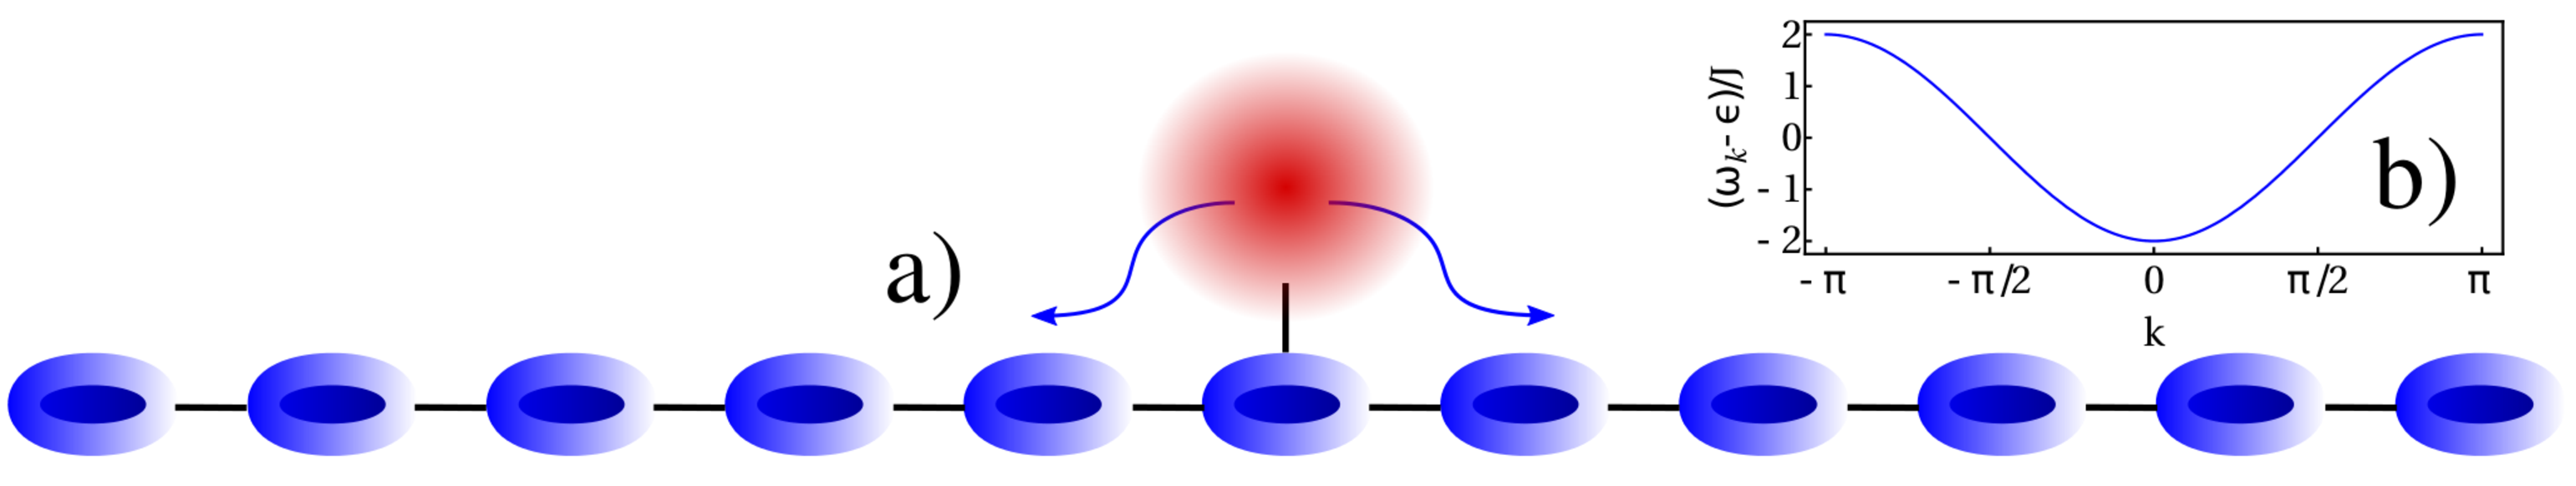
\includegraphics[width=1\columnwidth]{fig1_imp_gimp.pdf}
\caption{ {\bf a) Scheme of the system.} In blue, the bosonic array. The impurity is represented as a blurred black circle. {\bf b) Dispersion relation for the bosonic array}.}\label{fig:scheme}
\end{figure}

This model can be described by several physical set-ups, such as photonic crystals \cite{Lodahl2015}, coupled superconducting resonators \cite{Liu2017}, etc. {\color{red}AQU\'I FALTAN (i) MATERIAL Y (ii) PAR\'AMETROS.}

%%%%%%%%%%%%%%%%%%%%%%%%%%%%%%%%%%%%%%%%%%
%%%%%%%%%%%%%%%%%%%%%%%%%%%%%%%%%%%%%%%%%%

\subsection{Single-particle eigenstates}

This model is analytically solvable in the single-excitation subspace. A complete basis is given by the scattering eigenstates $|\Psi_k\rangle$ \cite{Nori2008a} and the bound states $|\Psi_\pm\rangle$ \cite{Longo2010,Longo2011}. The former can be written as,
\begin{align}
\label{eq:scattering_states} 
|\Psi_k\rangle = & \Big [ \sum_{x<0}(e^{ikx}+r_k e^{-ikx})a_x^\dagger 
 +  \sum_{x\geq 0} t_k e^{ikx} a_x^\dagger 
%\\ 
%& 
+ d_k b^\dagger \Big]  |0\rangle.
\end{align}
The state $|0\rangle$ represents the vacuum state of the system ($a_x|0\rangle=b|0\rangle = 0$).
The coefficients 
 $t_k$ and $r_k$ are the  
 transmission and reflection amplitudes respectively
for an incident plane wave.  They are given by, 
\begin{align}
\label{eq:transmission}
t_k & =\frac{iv_k(\omega_k - \Delta)}{iv_k(\omega_k-\Delta)-g^2} \, , 
\\
\label{eq:reflection}
r_k&=t_k-1 
\\ 
d_k  &= \frac{g t_k}{\omega_k-\Delta} \,
\label{eq:d_scattering_states}.
\end{align} 
On the other hand, the bound states read
\begin{equation}
 |\Psi_\pm\rangle =  N_\pm \left(\sum_x e^{-\kappa_\pm |x|} a_x^\dagger + d_\pm b^\dagger\right)|0\rangle.\label{eq:bound_states}
\end{equation} 
Here, $N_\pm$ is a normalization constant, $1/\kappa_\pm$ is the localization length, and $d_\pm$ is  the impurity amplitude. The energy of $|\Psi_\pm\rangle$ is $\omega_\pm = \epsilon - J(e^{-\kappa_\pm} + e^{\kappa_\pm})$. The expressions of $d_\pm$ and $N_\pm$, as well as the computation of $\kappa_\pm$, are shown in Appendix \ref{app:eigen}. Important enough, the localization lengths  $1/\kappa_\pm$, 
fix the properties for the bound states: the energies $\omega_\pm$, the impurity amplitudes $d_\pm$ and the normalization factors $N_\pm$.


We plot the bound states energies $\omega_\pm$ as a function of the coupling constant $g$, as well as the band limits for the scattering eigenstates in Fig. \ref{fig:E_bound}. 
Two cases are shown: (i) the impurity energy $\Delta$ at the middle of the band ($\Delta-\epsilon=0$, solid lines) and (ii) closer to the band bottom  ($\Delta-\epsilon=-J$, dotted-dashed lines). 
The bound states are localized (not propagating), thus they lie always outside the band limits.
As $g\to 0$, $\omega_{-(+)}$   approach the bottom (top) of the band.
If  the impurity splitting  is in the middle of the band, the energies of the bound states are  symmetric.
On the other hand, $\omega_-$ moves away from $\Delta$ faster than $\omega_+$ if $\Delta-\epsilon<0$, and vice versa. Therefore, the position of the impurity energy with respect to the band breaks the symmetry between $\omega_+$ and $\omega_-$.

\begin{figure}[thb!]
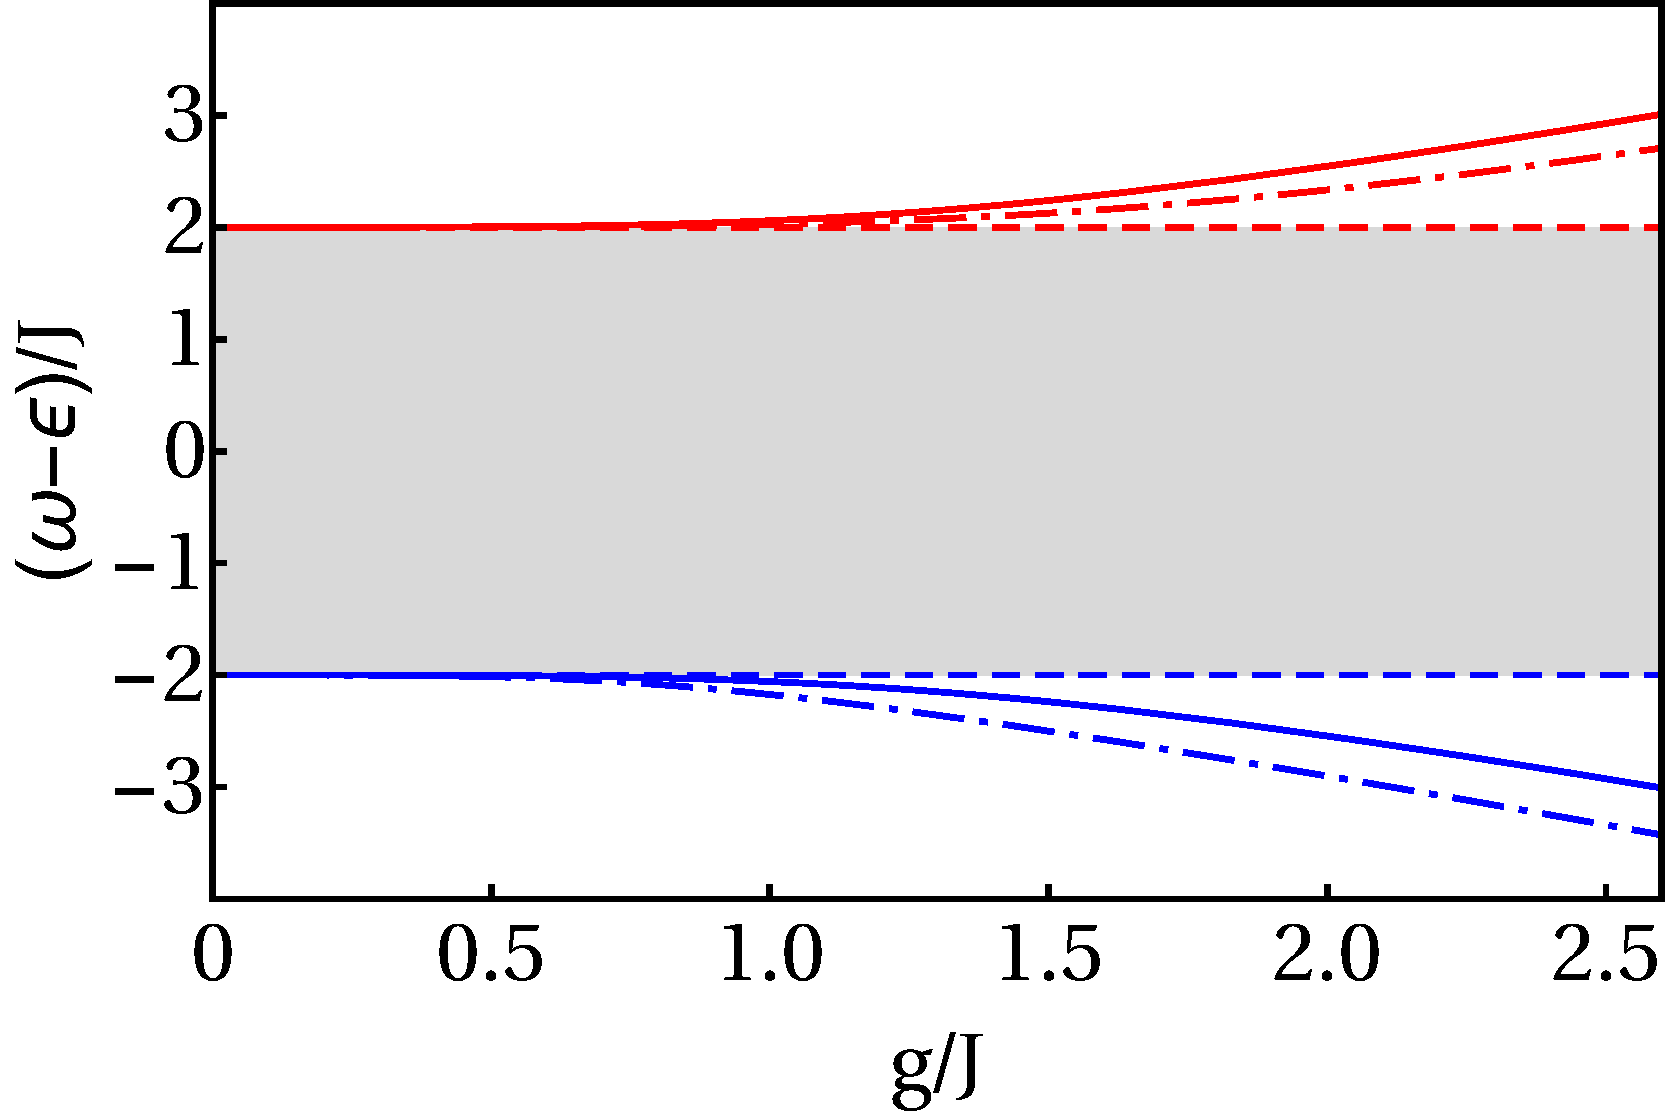
\includegraphics[width=1\columnwidth]{E_bound_all.pdf}
\caption{{\bf Bound states.} $(\omega_+-\epsilon)/J$ (solid, red line for $(\Delta-\epsilon)/J=0$ and dotted-dashed, red line for $\Delta-\epsilon=-J$) and $(\omega_--\epsilon)/J$ (solid, blue line for $\Delta-\epsilon=0$ and dotted-dashed, blue line for $\Delta-\epsilon=-J$) as a function of $g/J$. The red and blue dashed lines render the top and bottom band egdes respectively and the shaded zone represents the band.}\label{fig:E_bound}
\end{figure}
 

%%%%%%%%%%%%%%%%%%%%%%%%%%%%%%%%%%%%%%%%%%
%%%%%%%%%%%%%%%%%%%%%%%%%%%%%%%%%%%%%%%%%%

\section{Scattering dynamics}\label{sec:scatt}
For completeness, we review the single-particle scattering dynamics. This is a problem deeply studied in the literature \cite{Nori2008a, Fan2005a, Fan2005b, Guinea1987,Roy2016}.
Eq. \eqref{eq:transmission} reveals that, 
 when $\omega_k=\Delta$ there is full reflection ($T_k\equiv |t_k|^2=0$, $R_k\equiv |r_k|^2 = 1$). 
It is shown in Fig. \ref{fig:R}, where $R_k$ is illustrated with respect to $(\omega_k-\epsilon)/J$ and $(\Delta-\epsilon)/J$ for coupling $g=J/2$. 
Considering the  input as a single-photon-spectroscopy probe, we could be tempted to argue that, like in the scattering, the impurity emission is also maximum at resonance.  We will show that, due to the presence of bound states, this is not the case. 

\begin{figure}[thb!]
\begin{center}
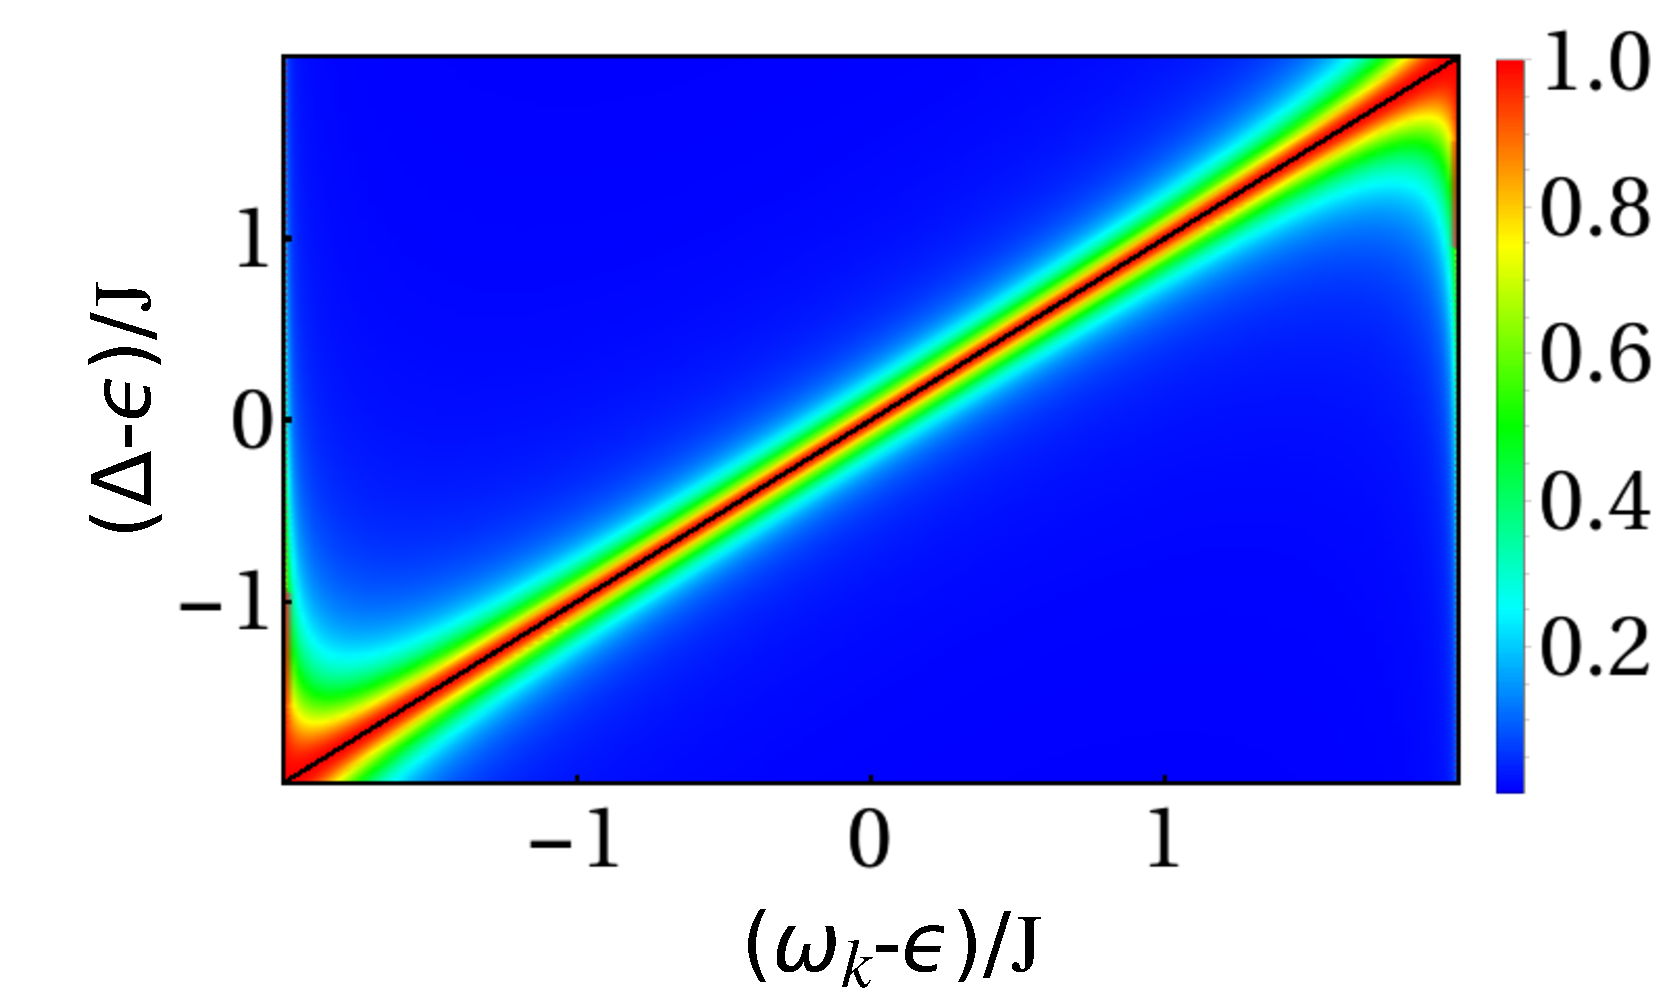
\includegraphics[width=1.\columnwidth]{R_vs_w_Delta_g_0_5.pdf}
\caption{{\bf Reflection probability.} $R_k$ as a function of $(\omega_k-\epsilon)/J$ and $(\Delta-\epsilon)/J$ for $g=J/2$. The black line is $\Delta=\omega_k$, where $R_k=1$; $R_k=1$, also at the band edges (Eq. \eqref{eq:transmission}).}\label{fig:R}
\end{center}
\end{figure}

%%%%%%%%%%%%%%%%%%%%%%%%%%%%%%%%%%%%%%%%%%
%%%%%%%%%%%%%%%%%%%%%%%%%%%%%%%%%%%%%%%%%%

\section{Spontaneous decay}\label{sec:spontaneous_decay}

We discuss now  the spontaneous emission.
In our studies, the  initial condition is $|\Psi(0)\rangle = b^\dagger |0\rangle$. Spanning this state in  scattering and bound eigenstates, Eqs. \eqref{eq:scattering_states} and \eqref{eq:bound_states}, the state at time $t$ is
\begin{align}
|\Psi(t)\rangle = & \frac{1}{2\pi}\int_{-\pi}^\pi dk\;c_ke^{-i\omega_k t}|\Psi_k\rangle \nonumber \\
 + & c_+ e^{-i\omega_+ t} |\Psi_+\rangle + c_- e^{-i\omega_- t} |\Psi_-\rangle, \label{eq:psi(t)}
\end{align}
with
\begin{align} \label{eq:ck}
c_k &  = \frac{iv_k g}{iv_k(\omega_k - \Delta) + g^2},\\
\label{eq:cpm}
c_\pm & =  \left(\frac{1+e^{-2\kappa_\pm}}{1-e^{-2\kappa_\pm}}+\frac{g^2}{(\omega_\pm - \Delta)^2}\right)^{-\frac{1}{2}} \frac{g}{\omega_\pm - \Delta}.
\end{align}

%%%%%%%%%%%%%%%%%%%%%%%%%%%
%%%%%%%%%%%%%%%%%%%%%%%%%%%
\subsection{Energy shift}

%The conserved energy of $|\Psi(t)\rangle$ is $\langle H\rangle (t) = \langle H\rangle (0) = \Delta$. Thus,
We want to calculate the mean energy of the emitted photon. For that, we first notice that $\Delta$ can be rewritten using that $\langle H\rangle$ is
\begin{equation}\label{eq:H(t)}
\langle H\rangle = \Delta  = \frac{1}{2\pi}\int_{-\pi}^\pi dk |c_k|^2 \omega_k + |c_+|^2 \omega_+ + |c_-|^2 \omega_- \, .
\end{equation}
The  average energy for the propagating field  is
\begin{equation}
\omega_\text{ph} \equiv \frac{\int_{-\pi}^\pi dk |c_k|^2 \omega_k/2\pi}{\int_{-\pi}^\pi dk |c_k|^2/2\pi} = \frac{\int_{-\pi}^\pi dk |c_k|^2 \omega_k/2\pi}{(1-P_\text{lig})},
\end{equation}
with $P_\text{lig} \equiv |c_+|^2 + |c_-|^2$.  
Using Eq. \eqref{eq:H(t)} the latter can be written in a more convenient way
\begin{equation}
\omega_\text{ph} =\frac{\Delta - |c_+|^2 \omega_+ - |c_-|^2 \omega_-}{1-P_\text{lig}}, \label{eq:omega_ph}
\end{equation}
which tells that the energy of the emitted photon is typically different from $\Delta$ because of the presence of the bound states.

The energy of the photon $(\omega_\text{ph}-\epsilon)/J$ is plotted as a function of $(\Delta-\epsilon)/J$ in Fig. \ref{fig:E_ph} for different values of $g$. The closer $\Delta$ is to the band edges, the more $\omega_\text{ph}$ departs from $\Delta$.
The shift increases monotonically with the coupling $g$. Eventually, as $g/J\to\infty$, the emitted energy coincides with the middle of the band for all $\Delta$.
%Therefore, whenever $\Delta$ is not in the middle of the band, the impurity emits a photon with an energy different than $\Delta$ even though the scattering resonance frequency happens as $\omega_k=\Delta$.
%This  breaks the correspondence between scattering and emission spectra. 


\begin{figure}[thb!]
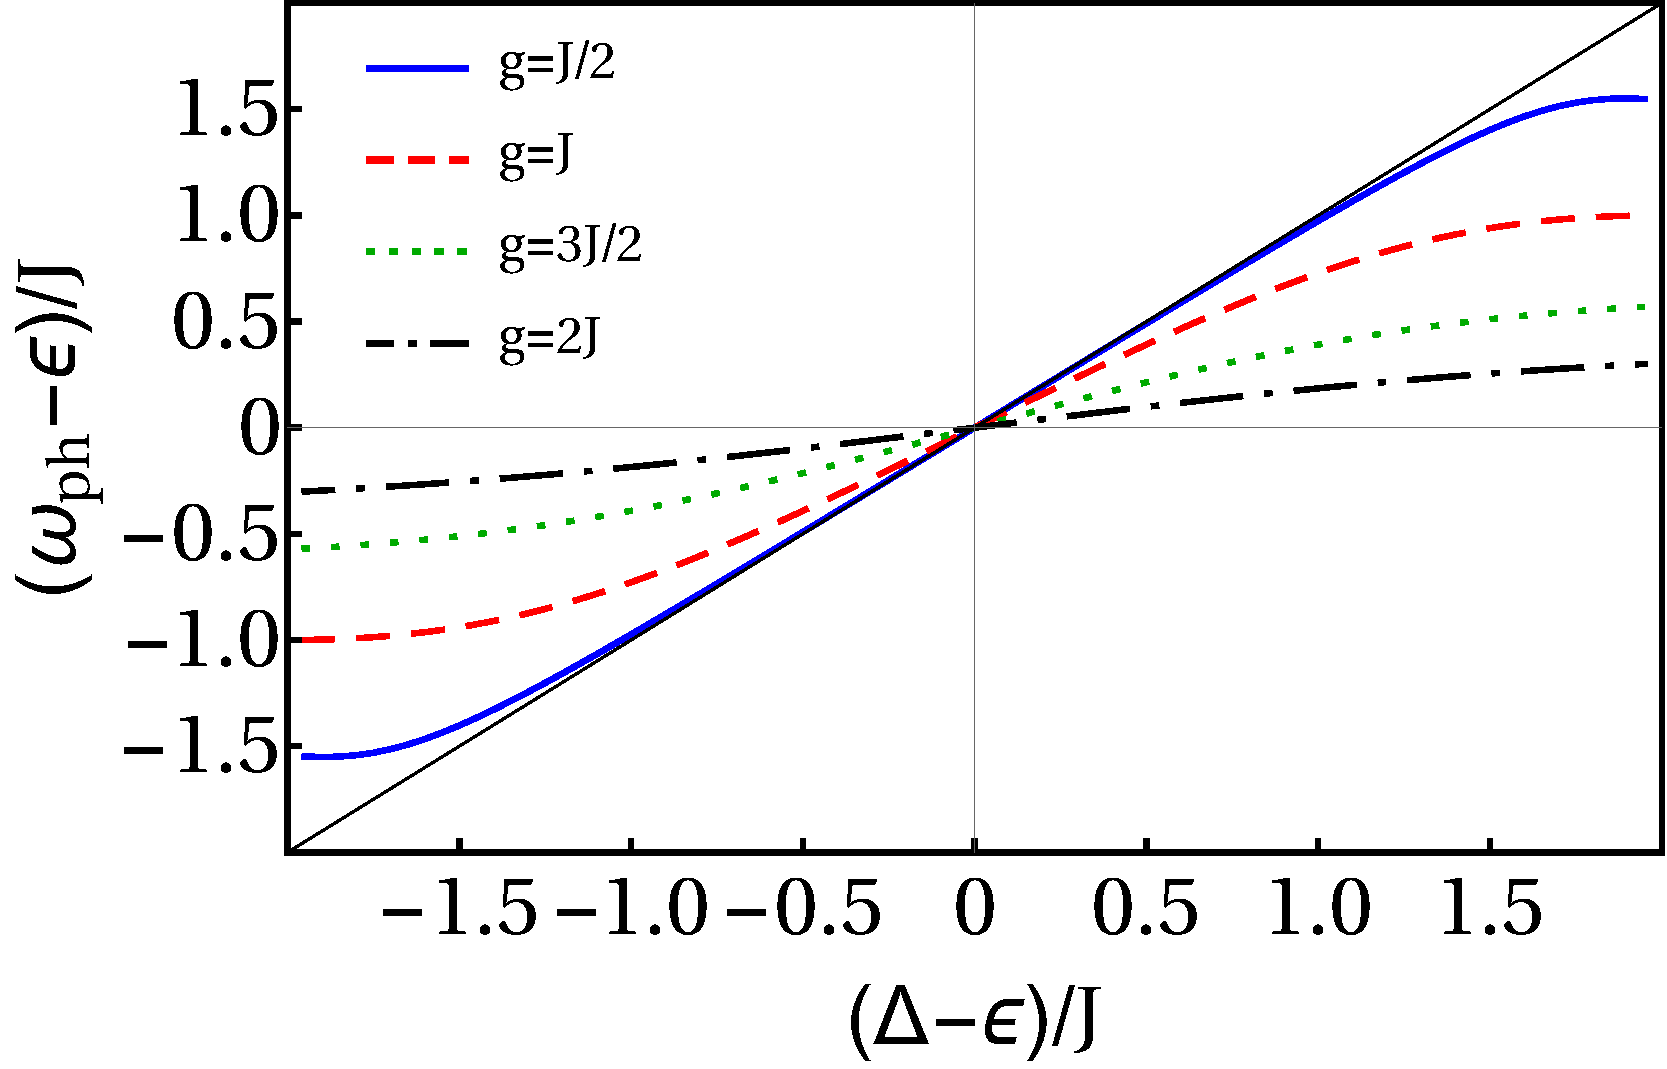
\includegraphics[width=1.0\columnwidth]{E_ph_vs_delta.pdf}
\caption{{\bf Mean photon energy.} Energy of the emitted photon $(\omega_\text{ph}-\epsilon)/J$ as a function of $(\Delta-\epsilon)/J$ for $g=J/2,J,3J/2,2J$. The straight line renders the diagonal $\omega_\text{ph}=\Delta$.% In the inset we show $\delta\omega_\text{ph}$ vs $g$ in log-log scale. The points are the numerical calculations and the solid lines fits to fourth order polynomials. The color code is the same as in the main plot ($\Delta=-1.5,-1.0,-0.5$ in blue, red and dark green respesctively, now from top to bottom)
}\label{fig:E_ph}
\end{figure}

Besides, we study the energy distribution of the emitted photon $|c_k|^2$. We plot it as a function of $(\omega_k-\epsilon)/J$ and $(\Delta-\epsilon)/J$ in Fig. \ref{fig:c_k} for $g=J/5$ and $g=J/2$ [panels a) and b), respectively]. If the coupling is small enough (left panel), the energy distribution is well peaked around $\omega_k=\Delta$. However, as $g$ increases (right panel), $|c_k|^2$ reaches its maximum for $\omega_k\neq\Delta$, being the difference larger as $\Delta$ is closer to one of the band edges. This deviation of the maximum away from $\Delta$ implies frequency shift of the emitted photon, as already seen in Eq. \eqref{eq:omega_ph} and Fig. \ref{fig:E_ph}. {\color{blue}We conclude that the existence of bound states breaks down the correspondence between scattering and emission spectra, since the energy of the emitted photon is different from the resonance energy of a scattering experiment, Eq. \eqref{eq:transmission}.}
%Therefore, we conclude that scattering and emission are not inverse problems but emission and absorption  are (as can be seen from the equality $c_k=d_k^*$, in Eqs.  \eqref{eq:d_scattering_states} and \eqref{eq:ck}).

\begin{figure}[thb!]
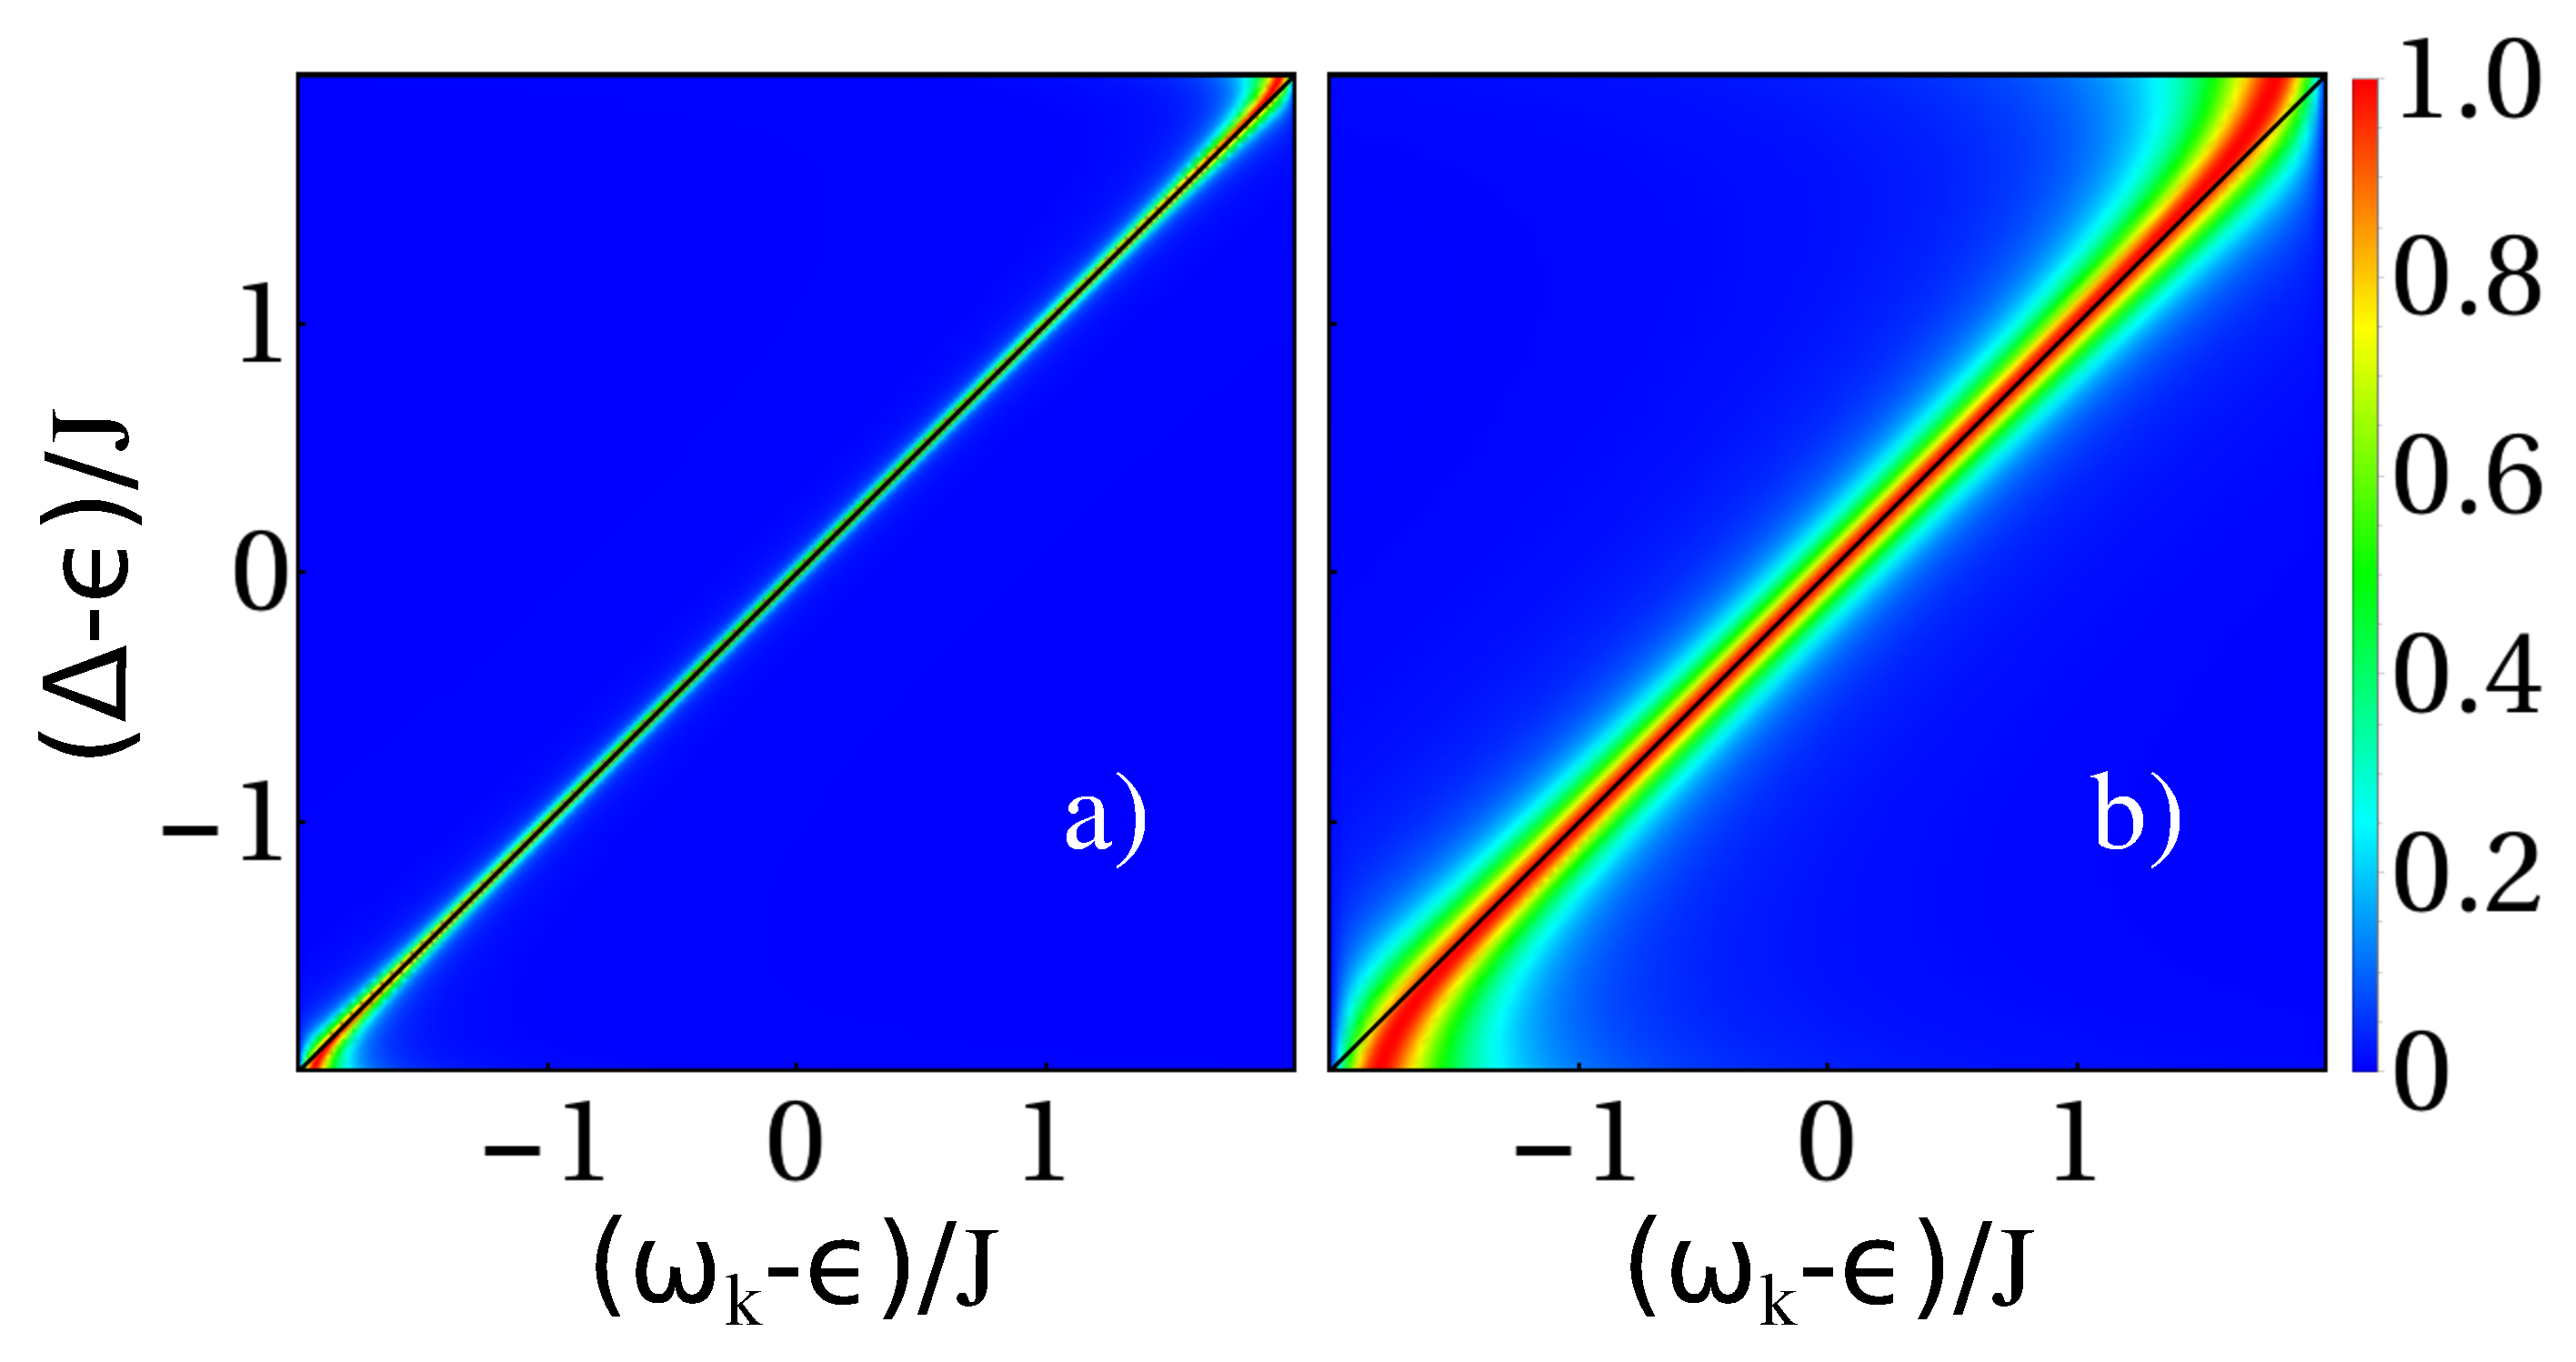
\includegraphics[width=1.0\columnwidth]{e_vs_w_Delta_g_0_2_0_5.pdf}
\caption{{\bf Emission energy distribution.} $|c_k|^2$ as a function $\omega_k/J$ and $\Delta/J$ for $\epsilon=0$ and a) $g=J/5$, b) $g=J/2$. The black line renders $\Delta=\omega_k$. We normalize $c_k$ such that $\text{max}_k(|c_k|^2)=1$.}\label{fig:c_k}
\end{figure}

{\color{blue}We now notice that at the middle of the band, $\Delta=\epsilon$, we have $\omega_\text{ph}=\Delta$. The reason is that $|c_+|^2(\omega_+-\Delta)=|c_-|^2(\Delta-\omega_-)$ at this point, Eq. \eqref{eq:omega_ph}. In addition, if the band gaps are sent to infinity, there are not bound states, so $\omega_\text{ph}=\Delta$.}
%In situations where the band limits are sent to infinity, there are not bound states and the impurity emits a photon peaked at its bare frequency, $\Delta$. In such a case, emission and scattering resonance occurs at the same energy, $\Delta$.  Whenever the bands are considered, as in our case,  the general  condition for vanishing frequency shift is $|c_+|^2(\omega_+-\Delta)=|c_-|^2(\Delta-\omega_-)$, Eq. \eqref{eq:omega_ph}. This condition is fulfilled if $\Delta$ is in the middle of the band, since $\omega_\pm$ move away from the band at the same rate (solid lines of Fig. \ref{fig:E_bound}) and the overlap with both eigenstates $|c_\pm|^2$ is the same, Cf. Eq. \eqref{eq:cpm}. 

Finally, we characterize the emission probability in propagating modes, $P_\text{emission}\equiv 1-P_\text{lig}$, in Fig. \ref{fig:P_emi}. Two effects are observed. First, the emission into bound states is negligible ($P_\text{emission} \cong 1$) in the range $g/J \ll1$. Increasing this ratio, $P_\text{emission}$ decreases. Besides, the closer is $\Delta$ to the band gap, the smaller is $P_\text{emission}$. Nevertheless, the emission probability is appreciable for really large values of the ratio: for instance $g/J \cong 2.5$ yields $P_\text{emission} \cong 0.25$ for the values of $\Delta$ considered in Fig. \ref{fig:P_emi}.

\begin{figure}[thb!]
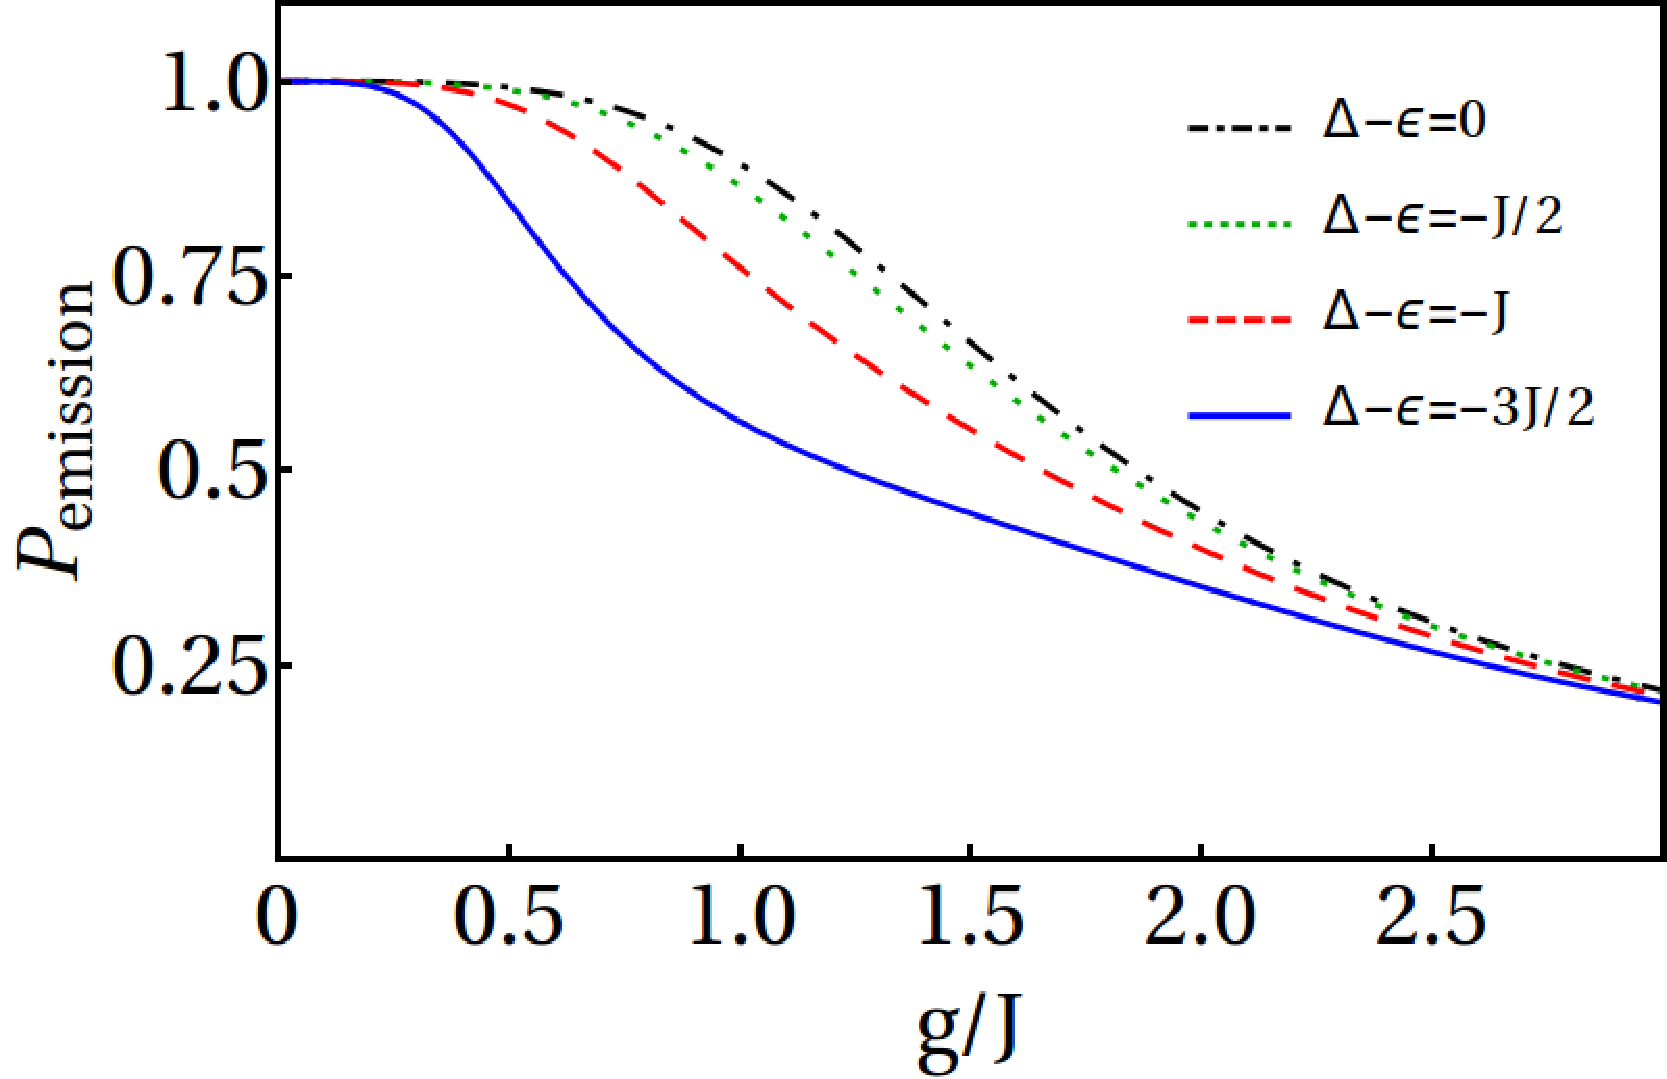
\includegraphics[width=1.0\columnwidth]{p_emission_a.pdf}
\caption{{\bf Probability of photon emission.} $P_\text{emission}$ as a function of $g/J$ for $\Delta-\epsilon=-3J/2,-J,-J/2,0$ from bottom to top (solid blue, dashed red, dotted green, and dot-dashed black, respectively).}\label{fig:P_emi}
\end{figure}

%%%%%%%%%%%%%%%%%%%%%%%%%%%%%%%%%%%%%%%%
%%%%%%%%%%%%%%%%%%%%%%%%%%%%%%%%%%%%%%%%

\subsection{Emitted field}

We now study the spatial profile of the emitted field by computing the amplitudes in position space, $\phi_x\equiv \langle 0|a_x|\Psi(t)\rangle$ [Cf. App.\ \ref{app:field}]. The photon probability distribution $|\phi_x|^2$ is shown in Fig. \ref{fig:w_n} at time $t=75/J$ for two values of the detuning: $\Delta-\epsilon=0$ (blue solid) and $-J$ (red dashed) for $g=J/5$. The vertical solid black lines represent $|x|=x_\text{max}\equiv v_\text{max}t$, defined in terms of the maximum group velocity $v_\text{max}= v_{k=\pi/2}=2J$. 

The propagator $|\phi_x|^2$ is mostly confined within the causal cone. It decays exponentially for $|x|>x_\text{max}$, as the free field scalar {\it propagator} \cite[Sect. 4.5]{Greiner-fq}, \cite[Sect. 2]{Peskin}. If $\Delta$ is in the middle of the band, the emitted photon has a momentum distribution peaked around $k=\pi/2$, where $v_k=v_\text{max}$. {\color{blue}If $\Delta\neq 0$, the velocity of the emitted photon is not peaked around $v_\text{max}$ and the maximum of $|\phi_x|^2$ is below $x_\text{max}$ (see the dashed red curve of Fig. \ref{fig:w_n}, where $\Delta-\epsilon=-J$)}. {\color{blue}Lastly, notice that the emitted photon would be well peaked around $|x_\text{max}|$ in position space independently of the value of $\Delta$ if the dispersion relation were linear.}


\begin{figure}[thb!]
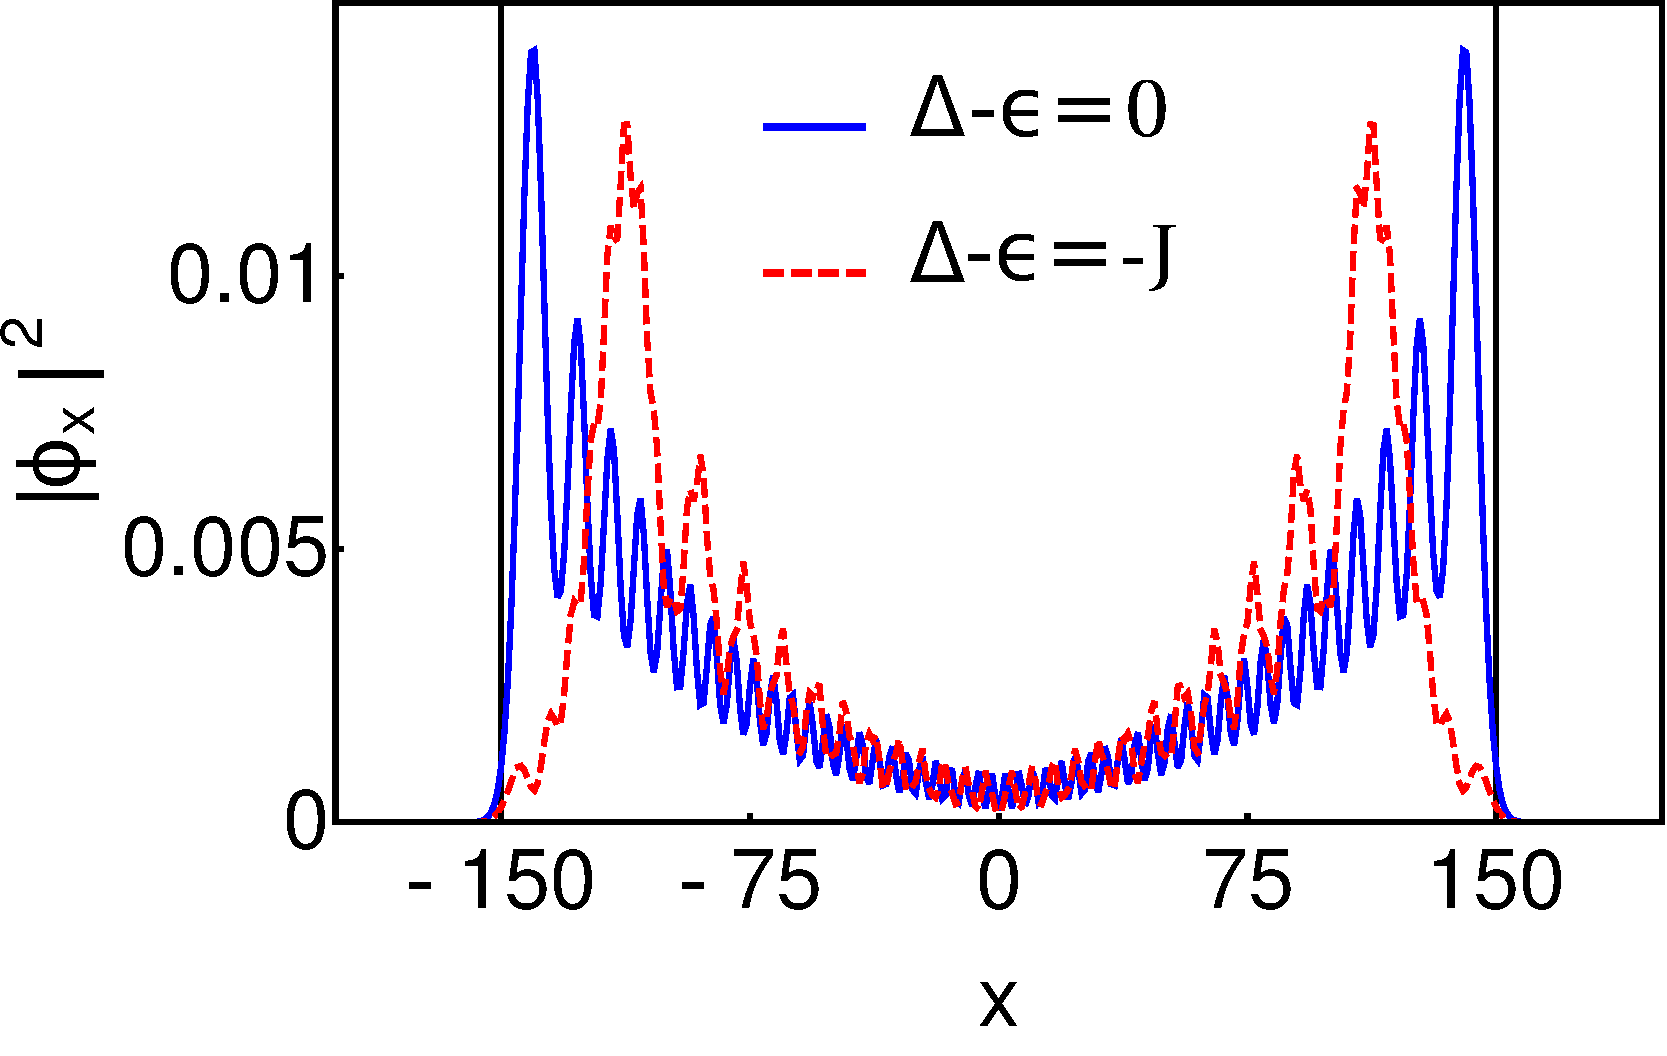
\includegraphics[width=1.0\columnwidth]{wx_g_0_2_Delta_0_-1.pdf}
\caption{{\bf Field distribution.} $|\phi_x|^2$ as a function of $x$ at time $t=75/J$ for $\Delta-\epsilon=0$ (solid blue) and $\Delta-\epsilon=-J$ (dashed red), fixing $g=J/5$. The black solid vertical lines render the propagation limit $|x|=v_\text{max}t$, with $v_\text{max}=v_{k=\pi/2}=2J$.}\label{fig:w_n}
\end{figure}

%%%%%%%%%%%%%%%%%%%%%%%%%%%%%%%%%%%%%%%%
%%%%%%%%%%%%%%%%%%%%%%%%%%%%%%%%%%%%%%%%


\subsection{Impurity dynamics}

%We analyze the time evolution of the amplitude of the excited state of the impurity, $c_1(t)$. 
%Using Eq. \eqref{eq:psi(t)} we obtain
{\color{blue}We finish with a detailed study of the impurity dynamics. From Eq. \eqref{eq:psi(t)}, we extract the time dependence of the impurity excited state amplitude}
\begin{equation}
\label{eq:qubit_amplitude}
c_1(t) \equiv
\langle 0|b|\Psi(t)\rangle 
 =
c_1^\text{s}(t) + 
c_1^\text{b}(t) \, .
\end{equation}
{\color{blue}Here, we find convenient to split the contribution from the scattering and bound states: $c_1^\text{s}(t) = \int_{-\pi}^\pi dk |c_k|^2 e^{-i\omega_k t}/2\pi$ and $c_1^\text{b}(t) = \sum_{\alpha=\pm}|c_\alpha|^2 e^{-i\omega_\alpha t}$.}
%where he have explicitly split the contribution to the decay due to coupling to propagating modes,  $c_1^\text{s}(t) = \int_{-\pi}^\pi dk |c_k|^2 e^{-i\omega_k t}/2\pi$, and to  bound states, $c_1^\text{b}(t) = \sum_{\alpha=\pm}|c_\alpha|^2 e^{-i\omega_\alpha t}$.

%This decay has already been studied in \cite{Lombardo2014} when $\Delta$ is in the middle of the band and in \cite{Garmon2013} as $\Delta$ is close to one of the band edges. We generalize these works, studying how the impurity decays as a function of the energy with respect to the photonic band.

First, we focus on  $c_1^\text{s}(t)$:
\begin{equation}
c_1^\text{s}(t) =  e^{-i\epsilon t}\frac{4g^2}{\pi J^2}\int_{-1}^1 dy\; F(y)e^{i2yJt}, \label{eq:c_sc_app}
\end{equation}
with
\begin{equation}
F(y)=\frac{\sqrt{1-y^2}}{4(1-y^2)\left((\Delta-\epsilon)/J+2y\right)^2+(g/J)^4}.\label{eq:F}
\end{equation}
\begin{figure}[thb!]
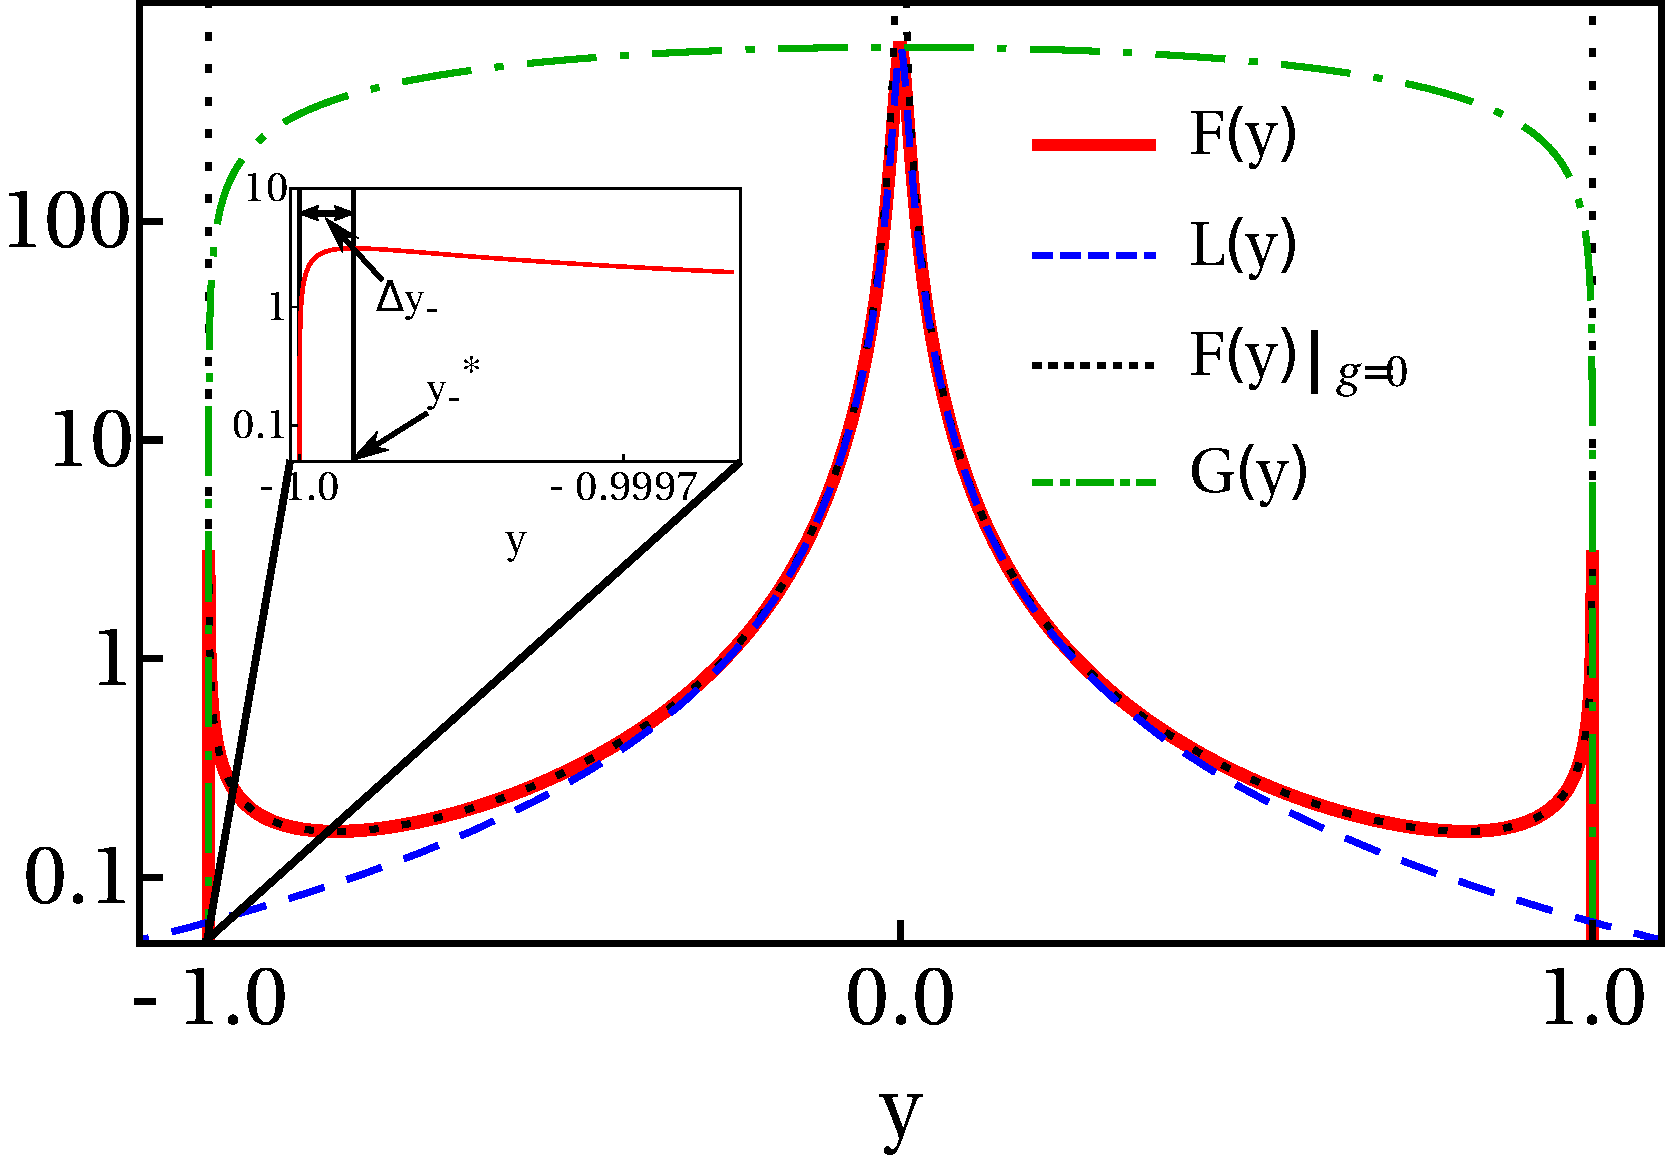
\includegraphics[width=1.0\columnwidth]{integrand_inset_Delta_0_g_0_2.pdf}
\caption{{\bf Integrand.} Kernel $F(y)$ for $g=J/5$ (red, solid), Lorentzian approximation (blue, dashed), $F(y)$ for $g=0$ (black, dotted), and $G(y)$ (Eq. \eqref{eq:G}, black, dotted-dashed). In the inset, we zoom $F(y)$ around $y=-1$ to see $\Delta y_-$. We fix $\Delta=\epsilon$.}\label{fig:integrand}
\end{figure}
Thus, the behavior of $c_1^\text{s}(t)$ is determined by the kernel $F(y)$, which is related to the density of photonic states in terms of the dimensionless energy $y = \cos k$. This kernel is plotted in Fig. \ref{fig:integrand}. At sufficiently long times, the oscillating term $e^{i2yJt}$ cancels out any smooth contribution from $F(y)$ to $c_1^\text{s}(t)$. %Fig. \ref{fig:qubit_dynamics} will show that this arguments provides accurate results almost from the initial time.
Therefore, the relaxation dynamics is governed by the sharpest peaks and the singularities of $F(y)$. Three parts of $F(y)$ give the main contributions: a Lorentzian peak, associated to a pole of $F(y)$ in the complex plane, two peaks appearing at $y_\pm^*$, with $y_\pm^*$ close to $\pm 1$, and the singular points at $y=\pm 1$, where the first derivative of $F(y)$ is discontinuous. All these features are seen in Fig. \ref{fig:integrand}.

The Lorentzian peak gives an exponential decay $c_1^\text{s}(t)\sim e^{-(i\varphi+1/2\tau_0)t}$. 
%{\color{red}The first order approximation of $\tau_0$ and $\varphi$ in $(g/J)^2$ recovers the result obtained by the Fermi golden rule, $\tau_0=J\sin k_\Delta/g^2$, with $k_\Delta$ such that $\omega_{k_\Delta}=\Delta$, and $\varphi=\Delta$ (details can be found in Appendix \ref{app:integrand})}. 
Figure \ref{fig:qubit_decay} compares the (numerical) exact results for $\tau_0$ and $\delta\varphi\equiv\varphi-\Delta$ with those obtained with the Lorentzian approximation of $F(y)$. {\color{blue}We also compare the results to the Fermi golden rule ones: $\tau_{0,\text{FGR}}=J\sin k_\Delta/g^2$, with $k_\Delta$ such that $\omega_{k_\Delta}=\Delta$, and $\varphi_\text{FGR}=\Delta$}. The Fermi golden rule perfectly matches the exact results when $\Delta$ is around the middle of the band, but {\color{blue}the corrections are} necessary as $\Delta$ gets closer to the band edges. %A breakdown of the Fermi golden rule has previously been seen in different impurity decay scenarios \cite{Petrosky2005,Tanaka2006,Garmon2009}.

{\color{blue}Secondly, we analyze the contribution of the peaks of $F(y)$ at $y_\pm^*$, with $y_\pm^*\simeq \pm 1$. Let us define their widths as $\Delta y_\pm\equiv |y_\pm^* \mp 1|$ (see inset of Fig. \ref{fig:integrand}). For short enough times, when $e^{i2Jyt}$ can be considered to be constant for $y\in (-1,-1+\Delta y_-)$ and $y\in (1-\Delta y_+,1)$, the kernel $F(y)$ can be approximated by itself for $g=0$ (black dotted curve in Fig. \ref{fig:integrand}). This effective kernel diverges as $1/\sqrt{1-y^2}$ when $y\to\pm 1$. This kind of singularity gives a $t^{-1/2}$ decay for the scattering amplitude. More precisely, $c_1^\text{s}(t)\sim t^{-1/2}(a e^{-i2Jt} + b e^{i2Jt})$, where the constants $a$ and $b$ are given in Appendix \ref{app:integrand}. However, for long enough times,  $e^{i2Jty}$ is not constant and we have to consider the full kernel with $g\neq 0$ and the  $\sqrt{1-y^2}$ divergence disappears. The peaks give an exponential decay as $e^{-t/\tau_{1,+}}$ and $e^{-t/\tau_{1,-}}$, $c_1^\text{s}(t)\sim t^{-1/2}(a e^{-i2Jt}e^{-t/2\tau_{1,-}} + b e^{i2Jt}e^{-t/2\tau_{1,+}})$, with $\tau_{1,\pm} = (4 \Delta y_\pm)^{-1}$.

Eventually, these exponential contributions vanish.  The only surviving contribution comes from the singularities at the band edges. There, $F(y)$ is not differentiable, with zero-width in $y-$space, so it provides a non-exponential (power-law) contribution to  $c_1^\text{s}(t)$ \cite{Khalfin1958,Fonda1978,Hack1982,Gaveau1995}, which dominates for  $t\gg \tau_0,\tau_{1,\pm}$. Calculations, detailed in Appendix \ref{app:integrand}, show that this contribution is $c_1^\text{s}(t)\sim t^{-3/2}\cos (2Jt-3\pi/4)$, which implies the contribution of the scattering states to the impurity population $P_1^\text{s}(t)\equiv |c_1^\text{s}(t)|^2$ decays with $t^{-3}$. This transition between $t^{-1}$ and $t^{-3}$ decay was already discussed in \cite{Garmon2013}, but they did not see the oscillating factors, since they took the impurity energy really close to the lower part of the band, neglecting the contribution of the upper bound state. This decay with $t^{-3}$ is quite common in impurity decay problems \cite{Chiu1977}, both for continuous systems \cite{Winter1961,GarciaCalderon2006} and for discrete ones \cite{Longhi2006a,Dente2008,Longhi2006b}.}


The contribution of the bound states $c_1^\text{b}(t)$ is much simpler: it gives an oscillatory term which, in the lossless case considered in this paper, persists for infinitely long times: $P_1^\text{b}(t)\equiv|c_1^\text{b}(t)|^2=|c_+|^4+|c_-|^4+2|c_+c_-|^2\cos((\omega_+-\omega_-)t)$, \cite{Gaveau1995,Lombardo2014}.

\begin{figure}[thb!]
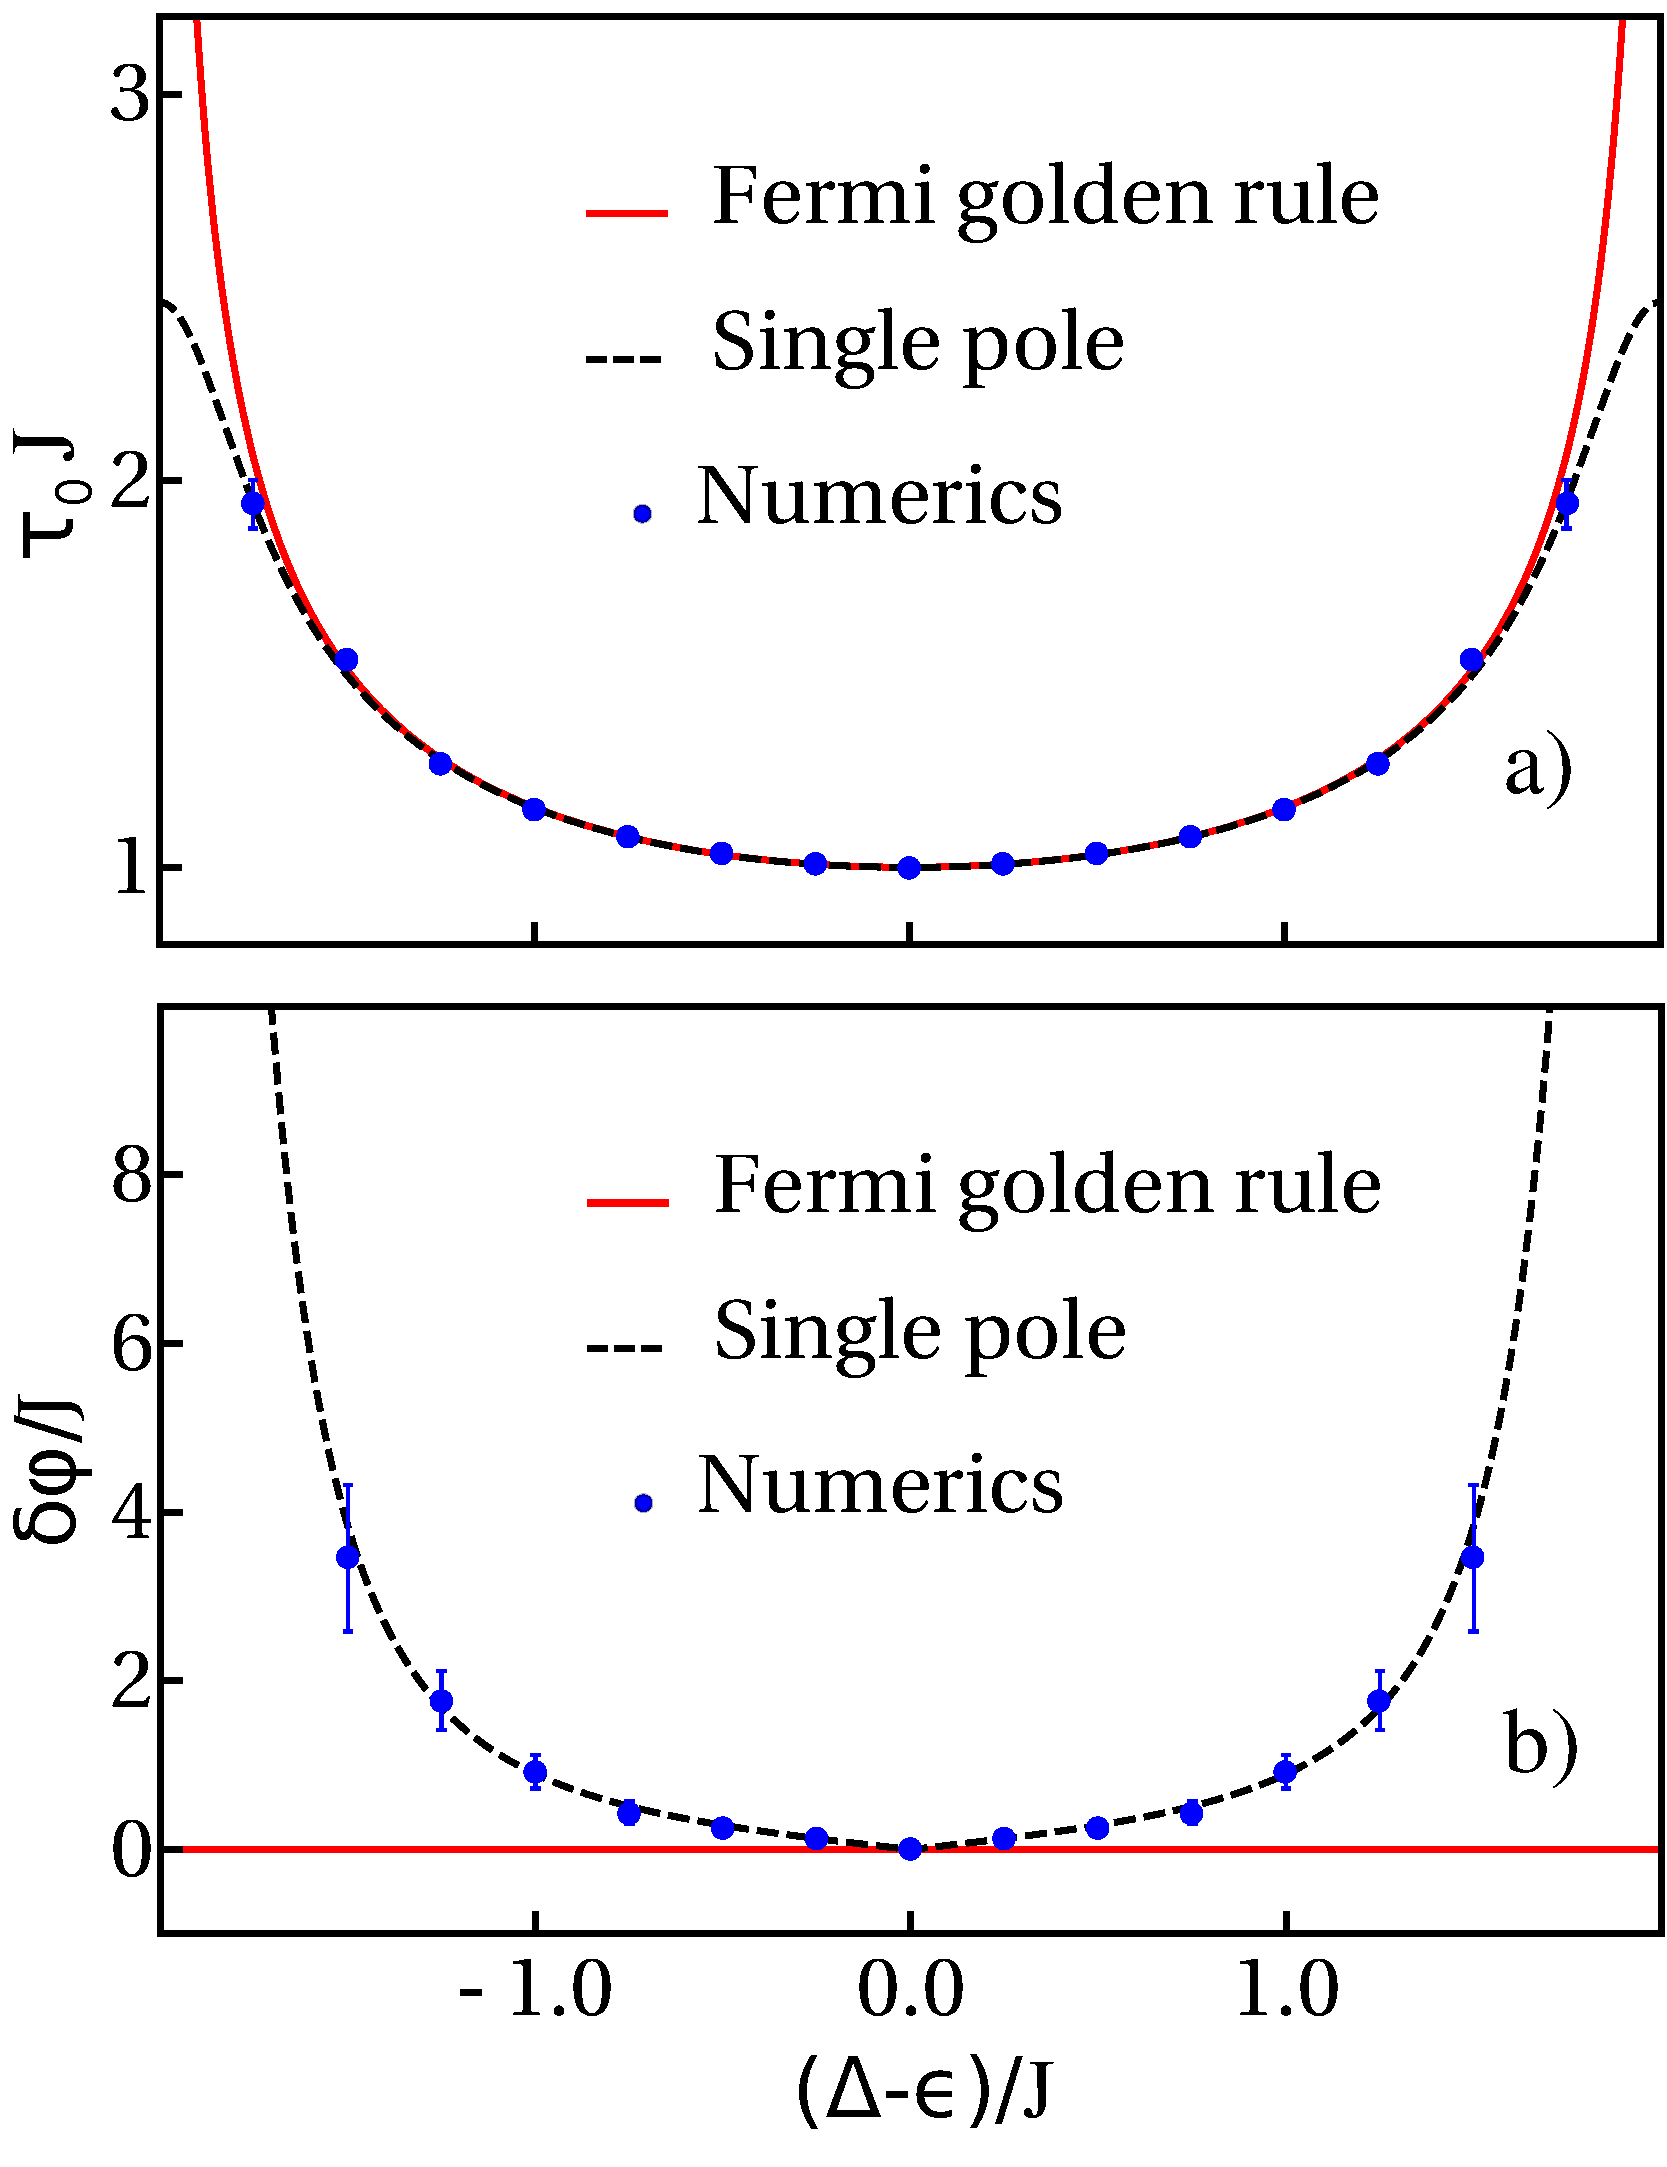
\includegraphics[width=1.0\columnwidth]{gamma_phi_g_0_3.pdf}
\caption{{\bf Exponential decay.} a) $\tau_0/\tau_{0,\text{FGR}}(\Delta-\epsilon=0)$ and b) $\delta\varphi/J$ depending on the position of the impurity energy with respect to the band for $g=3J/10$ and $\epsilon=0$. {\color{blue}We divide $\tau_0$ by the decay time given by the Fermi Golden rule at the middle of the band, $\tau_{0,\text{FGR}}(\Delta-\epsilon=0)$. The red solid curve and the black dashed one correspond to the Fermi Golden rule and to the single-pole approximation, respectively.} The blue points are computed numerically. As seen, the single-pole approximation works better close to the band egdes, whereas in the middle of the band both calculations converge.}\label{fig:qubit_decay}
\end{figure}


\begin{figure}[thb!]
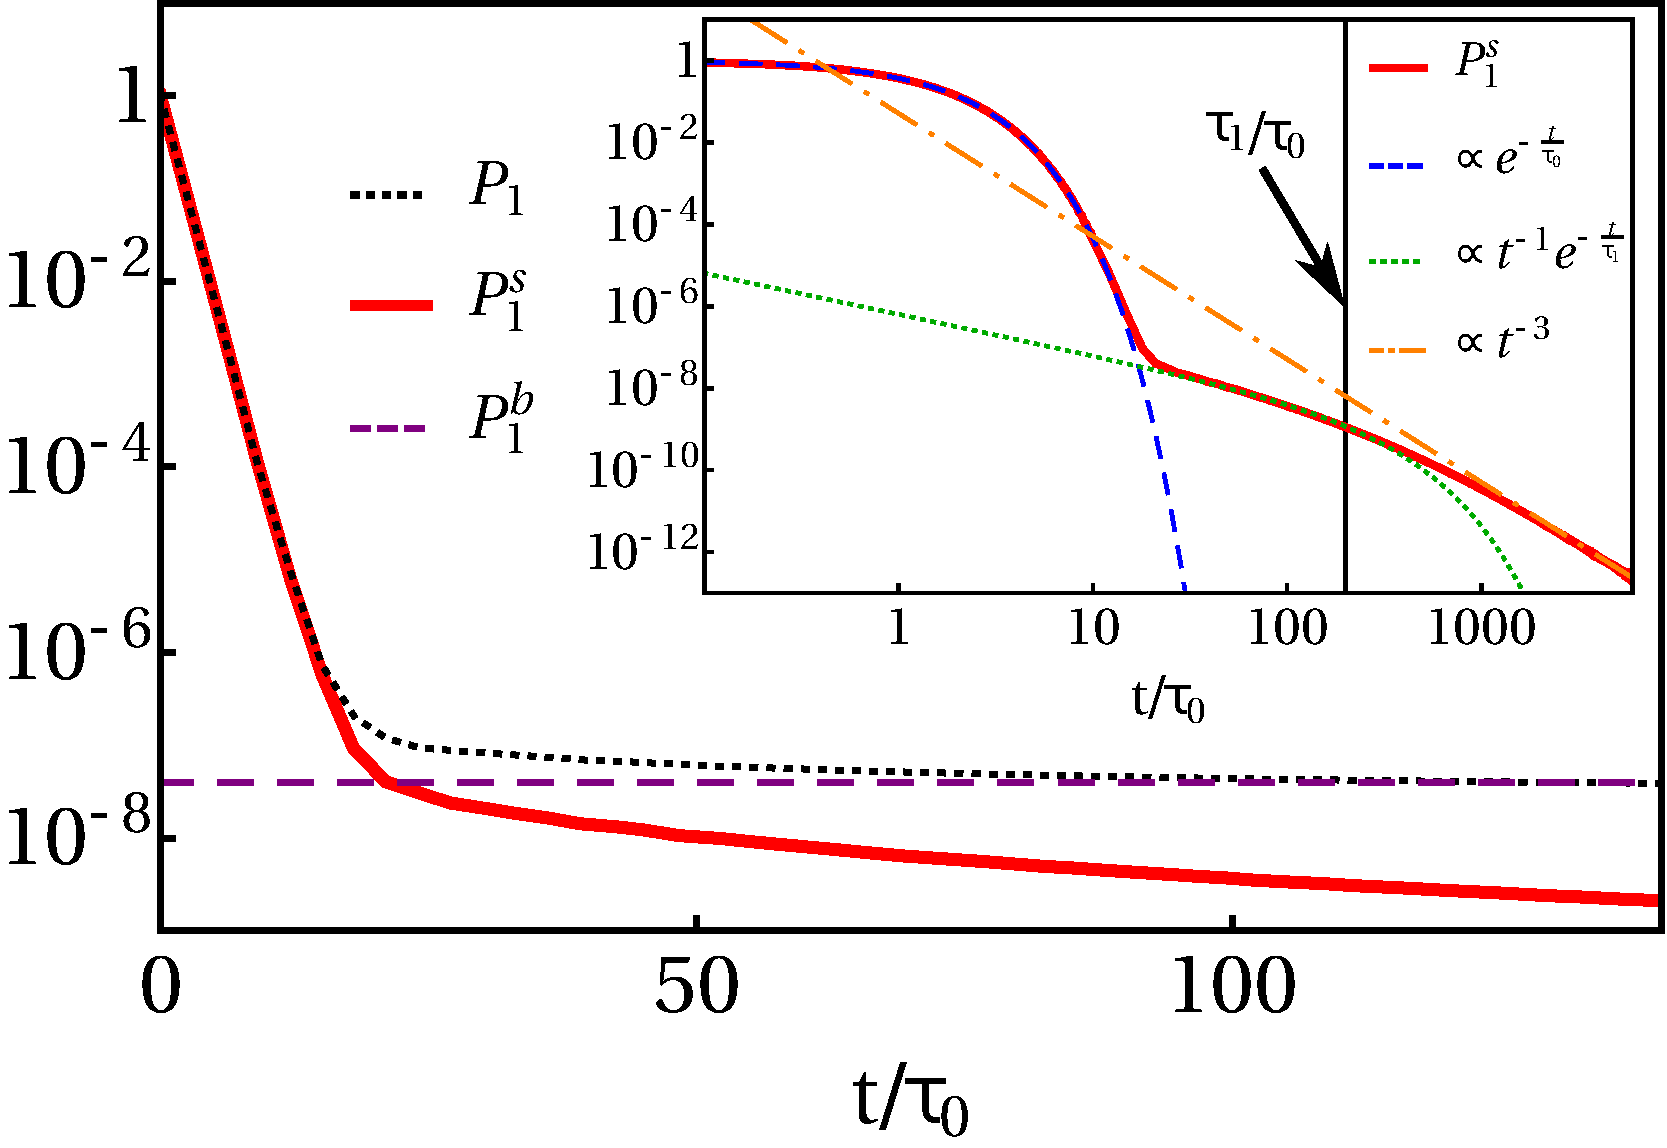
\includegraphics[width=1.0\columnwidth]{P_Delta_0_g_0_2.pdf}
\caption{{\bf Impurity dynamics.} $P_1(t)$ (black, dotted), $P_1^\text{s}(t)$ (red, solid), and $P_1^\text{b}(t)$ (purple, dashed) for $\Delta-\epsilon=0$ and $g=J/5$ in logarithmic scale. In the inset we show $P_1^\text{s}(t)$ in log-log scale with the three contributions: the exponential decay (blue, dashed), the power-law with $t^{-1}$ (green, dotted), and the decay with $t^{-3}$ (orange, dotted-dashed). We remark that this $t^{-3}$ contribution just makes sense in the infinite time limit, when the other contributions have already decayed. Notice that we remove the oscillations in all the curves for the sake of clarity.}\label{fig:qubit_dynamics}
\end{figure}

{\color{blue}We sum up all this information in Fig.\ \ref{fig:qubit_dynamics}, where we plot the impurity dynamics for $\Delta-\epsilon=0$ and $g=J/5$, using logarithmic scale. 
We remove the oscillations coming from the different contributions ($ae^{-i2Jt}+be^{i2Jt}$ from the peaks around $y_\pm^*$, $\cos(2Jt-3\pi/4)$ from the singularities at $y=\pm 1$, and $\cos((\omega_+-\omega_-)t)$ from $c_1^\text{b}(t)$) for the sake of clarity. The population $P_1(t)\equiv|c_1(t)|^2$ is drawn as a black, dotted curve. For the chosen parameters, $\tau_0\ll \tau_{1,\pm}$. Then, $P_1(t)$ first decays as $e^{-t/\tau_0}$. In addition, the bound-state term dominates over the remaining contributions from the scattering states, so, after a transient period, $P_1(t)$ achieves the stationary regime of $P_1^\text{b}(t)$ (purple, dashed curve; remind that we are not showing the oscillations). We also show $P_1^\text{s}(t)$ in the red solid curve. After the initial exponential decay with $e^{-t/\tau_0}$, where $P_1^\text{s}(t)\simeq P_1(t)$, it decays sub-exponentially. To see the different contributions to this sub-exponential decay more clearly, we plot it in the inset in log-log scale. It initially decays exponentially as $e^{-t/\tau_0}$, followed by a decay with $t^{-1}$ for $\tau_0\ll t\ll \tau_1$ (as $\Delta-\epsilon=0$, $\tau_1\equiv\tau_{1,+}=\tau_{1,-}$). Once $t\gtrapprox \tau_1$ we have $e^{-t/\tau_1}$, and, eventually, as $t\gg\tau_1$, it goes with $t^{-3}$. The agreement between the analytical prediction (orange, dotted-dashed curve) and the exact (numerical) integration is really good in this limit, as well as the oscillation with $\cos^2(2Jt-3\pi/4)$ (not shown).}

\section{Conclusions}\label{sec:conclusions}

{\color{blue}Spontaneous decay and scattering are not symmetric problems if there are bound states, since the scattering resonance frequency differs from the spontaneous emission frequency. We have also seen that the profile of the emitted photon strongly depends on the energy of the impurity with respect to the photonic band. Lastly, the presence of bound states makes the impurity dynamics nontrivial, with three dynamical regimes: Exponential decay, power-law, and oscillatory asymptotic regime. Even though the population at the power-law tail is very small, it has been measured in different contexts, as dissolved organic materials \cite{Rothe2006}}.

Some features, such as the spectroscopic shifts in the spontaneously emitted photons can be detectable by tuning up and down the frequency of the qubit with respect to the band edge. For time-domain experiments and probing the qubit dynamics, we suggest using a more sophisticated protocol that (i) places the qubit at the right frequency, (ii) then excites it and after a finite time $t$ (iii) detunes the qubit and probes dispersively its excited state population. All of these ideas can be implemented in state-of-the-art setups with superconducting cavities and transmon qubits \cite{Liu2017} and also with quantum dots in photonic crystals \cite{Arcari2014,Sollner2015,Lodahl2015}.  

Finally, by tuning the parameters, the three regimes in the spontaneous emission could be detectable, e.g. in supercounditing layouts as the ones discussed in Sect. \ref{sec:model} \cite{Liu2017}.


\begin{acknowledgements}
We acknowledge 
support by the Spanish Ministerio de Economia y Competitividad within projects MAT2014-53432-C5-1-R, FIS2012-33022, and No. FIS2014-55867-P, the Gobierno
de Aragon (FENOL group), CAM Research Network QUITEMAD+,
and the European project PROMISCE.
\end{acknowledgements}

\appendix

\section{Bound States}\label{app:eigen}

%\subsection{Scattering states}

%We start by writing the coefficients of the scattering states (Eq. \ref{eq:scattering_states}). By solving the eigenvalue equation for $|\Psi_k\rangle$ one can obtain that the impurity amplitude $d_k$ is
%\begin{equation}
%d_k=\frac{g t_k}{\omega_k-\Delta}\label{eq:d_scattering_states}.
%\end{equation}
%This is how we obtain the value of $c_k=\langle \Psi_k|\sigma^+|0\rangle=d_k^*$, shown in the main text (Eq. \ref{eq:ck}).

%By imposing continuity of $|\Psi_k\rangle$ at the impurity position, the reflection amplitude is
%\begin{align}
%\label{eq:reflection} r_k & = t_k - 1.
%\end{align}

%\subsection{Bound states}

Let us introduce the expressions of the bound states (Eq. \eqref{eq:bound_states}). The impurity excited state amplitude $d_\pm$ is
\begin{equation}
d_\pm = \frac{g}{\omega_\pm - \Delta}.\label{eq:d_bound_states}
\end{equation}
In order to compute $\kappa_\pm$, we define $\eta_\pm \equiv e^{-\kappa_\pm}$ and use the eigenvalue equation $H|\Psi_\pm\rangle = \omega_\pm|\Psi_\pm\rangle$ \cite{Longo2011}
\begin{equation}\label{eq:eta}
\eta_\pm ^4 + \frac{\Delta-\epsilon}{J} \eta_\pm ^3 + \frac{g^2}{J^2} \eta_\pm ^2 - \frac{\Delta-\epsilon}{J} \eta_\pm - 1 = 0.
\end{equation}
This fourth degree algebraic equation has four solutions. However, we have two constrains: $\text{Re}(\kappa_\pm)>0$, because the photonic cloud is exponentially localized around the impurity, and $\text{Im}(\kappa_\pm)=0,\pi$, since $\omega_\pm = \epsilon - J(e^{-\kappa_\pm} + e^{\kappa_\pm}) \in \mathbb{R}$. There are just two solutions for $\eta_\pm$ fulfilling these restrictions.
The normalization factor is
\begin{equation}\label{eq:Npm}
N_\pm = \left(\frac{1+e^{-2\kappa_\pm}}{1-e^{-2\kappa_\pm}}+|d_\pm|^2\right)^{-1/2}.
\end{equation}
Finally, $c_\pm=\langle 0|\sigma^-|\Psi_\pm\rangle=(N_\pm d_\pm)^*$ can be obtained (Eq. \eqref{eq:cpm}), since we know both $d_\pm$ and $N_\pm$.

%\section{Power expansion of $\delta\omega_\text{ph}$}\label{app:wph}

%First of all, we have to compute $\eta_\pm$ by solving Eq. \ref{eq:eta}. Trivially, we realize that $\eta$ is an even function of $g$. Then, we expand $\eta_\pm$ in $g$:
%\begin{equation}\label{eq:eta_2}
%\eta_\pm\simeq \mp 1 + c_{2,\pm} (g/J)^2 + c_{4,\pm} (g/J)^4.
%\end{equation}
%Introducing this into Eq. \ref{eq:eta} and expanding the resulting equations up to fourth order:
%\begin{align}
%&\left(1-4c_{2,+}+2c_{2,+}\frac{\Delta-\epsilon}{J}\right)\frac{g^2}{J^2}\\
%&+\left(6c_{2,+}^2-2c_{2,+}-4c_{4,+}+(2c_{4,+}-3c_{2,+}^2)\frac{\Delta-\epsilon}{J}\right)\frac{g^4}{J^4} = 0\nonumber,\\
%&\left(1+4c_{2,-}+2c_{2,-}\frac{\Delta-\epsilon}{J}\right)\frac{g^2}{J^2}\\
%&+\left(2c_{2,-}+6c_{2,-}^2+4c_{4,-}+(3c_{2,-}^2 + 2c_{4,-})\frac{\Delta-\epsilon}{J}\right)\frac{g^4}{J^4} = 0\nonumber.
%\end{align}
%We get $c_{n,\pm}$ solving this system:
%\begin{align}
%&c_{2,\pm}=-\frac{J}{2(\Delta - \epsilon \mp 2J)},\\
%&c_{4,\pm}=\mp\frac{J^2}{8(\Delta-\epsilon \mp 2J)^2}.
%\end{align}
%Once we know $\eta_\pm$ (Eq. \ref{eq:eta_2}), we can calculate $\omega_\pm=\epsilon-2J(\eta_\pm^{-1}+\eta_\pm)$ and $|c_\pm|^2$ (Eq. \ref{eq:cpm}) up to fourth order:
%\begin{align}
%&\omega_\pm=\epsilon \pm 2J \pm  \frac{1}{4J(\Delta-\epsilon \mp 2J)^2}g^4,\\
%&|c_\pm|^2=\frac{(g/J)^4}{2J(2J\pm (\Delta-\epsilon))^3}.
%\end{align}
%Introducing this into the expression of $\delta\omega_\text{ph}$ (Eq. \ref{eq:omega_ph}) and expanding again up to fourth order:
%\begin{equation}
%\delta\omega_\text{ph}=\Delta-\frac{4(\Delta-\epsilon)}{((\Delta-\epsilon)^2-4J^2)^2}g^4 + \mathcal{O}\left(g^6/J^5\right),
%\end{equation}
%which is the formula we write in the main text (Eq. \ref{eq:omega_ph_4}).

\section{Emitted field}\label{app:field}

The profile of the emitted field $\phi_x(t)=\langle 0|a_x|\Psi(t)\rangle$ fulfills the following expression:
\begin{align}
\phi_x(t)& = \frac{1}{2\pi}\int_{-\pi}^\pi dk c_k e^{-i\omega_k t}\langle 0|a_x|\Psi_k\rangle \\
& + c_+ e^{-i\omega_+ t} \langle 0|a_x|\Psi_+\rangle+ c_- e^{-i\omega_- t} \langle 0|a_x|\Psi_-\rangle, \nonumber
\end{align}
where we have used Eq. \eqref{eq:psi(t)}. In order to compute the amplitude $\langle 0|a_x|\Psi_k\rangle$ we take the expression of $|\Psi_k\rangle$, Eq. \eqref{eq:scattering_states}, for $k>0$:
\begin{equation}
\langle 0|a_x|\Psi_k\rangle = \left\{ 
\begin{array}{c}
e^{ikx}+r_ke^{-ikx}\quad x<0,\\
t_k e^{ikx} \qquad\qquad\;\;\; x\geq 0.
\end{array}
\right.
\end{equation}
If $k<0$:
\begin{equation}
\langle 0|a_x|\Psi_k\rangle = \left\{ 
\begin{array}{c}
t_k e^{ikx} \qquad\qquad\;\;\; x< 0,\\
e^{ikx}+r_ke^{-ikx}\quad x\geq 0.
\end{array}
\right.
\end{equation}
Because of these terms, $|\phi_x(t)|^2$ shows oscillations in position space (Fig. \ref{fig:w_n}).

The amplitudes $\langle 0|a_x|\Psi_\pm\rangle$ are computed by projecting on $|\Psi_\pm\rangle$ (Eq. \eqref{eq:bound_states}):
\begin{equation}
\langle 0|a_x|\Psi_\pm \rangle= N_\pm e^{-\kappa_\pm |x|}.
\end{equation}



\section{Impurity dynamics: analyzing the integrand}\label{app:integrand}

%\begin{align}
%&c_1^\text{s}(t) =  e^{-i\epsilon t}\frac{4g^2}{\pi J^2}\int_{-1}^1 dy F(y)e^{i2yJt}\label{eq:c_sc_app},\\
%&F(y)=\frac{\sqrt{1-y^2}}{4(1-y^2)\left((\Delta-\epsilon)/J+2y\right)^2+(g/J)^4}.\label{eq:F}
%\end{align}
The integrand $F(y)$, Eq. \eqref{eq:F}, depicts a well peaked behavior, with a Lorentzian profile around a value $y$ far from the integration limits when $\Delta$ is far enough from the band edges and the coupling constant is small enough (see red, solid curve of Fig. \ref{fig:integrand}, with $g=J/5$ and $\Delta-\epsilon=0$). In such a case, we can substitute $F(y)$ by $L(y)\sim 1/((y-y_p)(y-y_p^*))$, being $y_p$ the pole corresponding to the peak of $F(y)$, with $-1<\text{Re}(y_p)<1$ and $\text{Im}(y_p)>0$. We extend the integration domain to $\pm\infty$. Then
\begin{equation}
c_1^\text{s}(t) = i8(g/J)^2 e^{-i\epsilon t}e^{i2y_p Jt}\text{Res}(F(y),y=y_p),
\end{equation}
By computing this numerically, we obtain the decay rate  $\tau_0 = (4J\;\text{Im}(y_p))^{-1}$ and the phase $\varphi = \epsilon - 2J\;\text{Re}(y_p)$, as shown in Figs. \ref{fig:qubit_decay} a) and b) respectively in the main text.

%\begin{figure}[thb!]
%\includegraphics[width=1.0\columnwidth]{../Figures/integrand_inset_Delta=0_g=0,2.pdf}
%\caption{{\bf Integrand.} Integrand $F(y)$ for $g=J/5$ and $\Delta-\epsilon=0$ (red, solid), the same for $\Delta-\epsilon=0$ and $g=0$ (blue, dashed) and $G(y)$ (Eq. \ref{eq:G}, black, dotted). In the inset, we zoom $F(y)$ around $y=-1$ to see $\Delta y_-$.}\label{fig:integrand}
%\end{figure}

When $t\gg \tau_0$, different regimes emerge. $F(y)$ has a sharp behavior for $y_\pm^*\simeq \pm 1$. Actually, it diverges when $y\to\pm 1$ if $g=0$. In order to take into account this contribution, we can approximate $F(y)$ by $F(y)|_{g=0}$ (see blue, dashed curve of Fig. \ref{fig:integrand})
\begin{equation}
c_1^\text{s}(t)\simeq \frac{4g^2}{\pi J^2}\int_{-1}^1 dy \frac{e^{i2yJt}}{4\sqrt{1-y^2}((\Delta-\epsilon)/J+2y)^2}.
\end{equation}
If $2\Delta y_\pm Jt\ll 1$, with $\Delta y_\pm=|y_\pm^*\mp 1|$ (already defined in the main text), the oscillatory term $e^{i2yJt}$ will not be sensitive to the difference between $F(y)$ and $F(y)|_{g=0}$ when $y$ is close to the edges and the approximation will work. As we are concerned in the contribution around $\pm 1$, we can approximate the integral as:
\begin{align}
c_1^\text{s}(t)  \simeq \frac{4g^2}{\sqrt{2}\pi J^2}&\left(\frac{J^2}{(\Delta-\epsilon-2J)^2}\int_{-1}^\infty dy \frac{e^{i2yJt}}{4\sqrt{1+y}}\right. \\
& \left.+ \frac{J^2}{(\Delta-\epsilon+2J)^2}\int_{-\infty}^1 dy \frac{e^{i2yJt}}{4\sqrt{1-y}}\right).\nonumber
\end{align}
These integrals are analytical
\begin{equation}
c_1^\text{s}(t)\simeq \frac{g^2}{2\sqrt{2\pi Jt}}\left(\frac{e^{-i2Jt}}{(\Delta-\epsilon-2J)^2}+\frac{e^{i2Jt}}{(\Delta-\epsilon+2J)^2}\right).\label{eq:csc_1}
\end{equation}
Then, $P_1^\text{s}(t)$ decays with $(Jt)^{-1}$ after the initial exponential decay if $\tau_0\ll t\ll \tau_{1,\pm}$, with $\tau_{1,\pm} = (4|\Delta y_\pm|)^{-1}$. We can rewrite the last expression by adding the decaying exponentials with $\tau_{1,\pm}$:
\begin{align}
c_1^\text{s}(t)\simeq \frac{g^2}{2\sqrt{2\pi Jt}}&\left(\frac{e^{-i2Jt}}{(\Delta-\epsilon-2J)^2} e^{-t/2\tau_{1,-}}\right. \nonumber \\
&\left. +\frac{e^{i2Jt}}{(\Delta-\epsilon+2J)^2} e^{-t/2\tau_{1,+}} \right).
\end{align}
In the case of the Fig. \ref{fig:qubit_dynamics}, $\Delta-\epsilon=0$, thus $\tau_{1,+}=\tau_{1,-}$.

Finally, if $t\gg \tau_0,\tau_{1,\pm}$, the only surviving contributions will be due to the singularities of $F(y)$ because the rapidly oscillating term $e^{i2yJt}$ cancels out the integrated contribution of any smooth part of the kernel. $F(y)$ is singular at $y=\pm 1$. Then, we can approximate the kernel by any function which behaves as $F(y)$ when $y=\pm 1$. We consider the function $G(y)$ (see Fig. \ref{fig:integrand}, black, dotted curve)
\begin{equation}
G(y)=\frac{\sqrt{1-y^2}}{(g/J)^4}.\label{eq:G}
\end{equation}
It is the same function as $F(y)$ neglecting the $y$-dependent part of the denominator. Then, if $t\gg \tau_0,\tau_{1,\pm}$
\begin{equation}
c_1^\text{s}(t) \simeq  \frac{4J^2}{\pi g^2}\int_{-1}^1 dy \sqrt{1-y^2} e^{i2yJt}=\frac{2J}{g^2 }\frac{J_1(2Jt)}{t},
\label{eq:c_sc_bessel}
\end{equation}
being $J_1$ the first kind Bessel function with $n=1$. As $t\to\infty$, $J_1(2Jt)\to (\pi Jt)^{-1/2}\cos(2Jt-3\pi /4)$, so $P_1^\text{s}(t)$ decays with $(Jt)^{-3}$ in the long-time limit.

%If we consider $|n|\gg 1/\text{Re}(\kappa_\pm)$ and $n>0$:
%\begin{align}
%\phi_n(t)& \simeq \frac{1}{\sqrt{2\pi}}\int_{-\pi}^0 dk c_k e^{-i\omega_k t}(e^{ikn} + r_ke^{-ikn}) \nonumber\\
%& + \frac{1}{\sqrt{2\pi}}\int_0^\pi dk c_k e^{-i\omega_k t}t_ke^{ikn}.
%\end{align}

%\section{Non-Markovianity}
%
%As said in the main text, the qubit dynamics is not the typical exponential decay. In this appendix, we argument why this dynamics is, in addition, non-Markovian.\newline
%
%\begin{figure}[thb!]
%\includegraphics[width=1.0\columnwidth]{../Figures/Gamma_qb_Delta=0,80_g=0,30.pdf}
%\caption{{\bf Qubit dynamics.} $\Gamma$ for $\Delta=0.80$ and $g=0.30$ in logarithmic scale.}\label{fig:Gamma}
%\end{figure}
%
%It is possible to modelize the qubit dynamics as a Lindblad one without Hamiltonian term, leading to
%\begin{equation}
%\frac{d|c(t)|^2}{dt} = -\Gamma(t) |c(t)|^2,
%\end{equation}
%being $\Gamma(t)$ the decay rate. If $\Gamma(t)=\Gamma_0$ for all $t$, we have the typical exponential behavior. However, this is not our case. As introduced by Rivas et al in \cite{Plenio2010}, we talk about Non-Markovian dynamics if $\Gamma(t)<0$. Since our dynamics has revivals, we can anticpate that it will be non-Markovian. We show $\Gamma(t)$ for $\Delta=0.80$ and $g=0.30$ (same parameters as in Fig. \ref{fig:qubit_dynamics}) in Fig. \ref{fig:Gamma}. As seen, in the beginning, corresponding to the initial decay, $\Gamma(t)>0$. However, $\Gamma(t)$ clearly takes negative values, following oscillations in the stationary regime, in the same way as $P_\text{qb}(t)$, as expected. So, we conclude that this system has a Non-Markovian behavior.


\bibliographystyle{apsrev4-1}
\bibliography{scattering_eduardo} 

\end{document}
